\documentclass{article}
\linespread{.5}
\usepackage[a4paper, margin=3mm, landscape]{geometry}
\usepackage{multicol}
\usepackage{xcolor}
\usepackage{enumitem}
\usepackage{amsmath}
\usepackage{amsfonts}
\usepackage{listings}
\usepackage{soul}
\usepackage{graphicx}

\pdfinfo{
    /Title (CS2106.pdf)
    /Creator (TeX)
    /Producer (pdfTeX 1.40.0)
    /Author (Vincent Pang)
    /Subject (CS2106)
    /Keywords (CS2106, nus, cheatsheet, pdf)
}

\graphicspath{ {./img/} }

\pagestyle{empty}
\setcounter{secnumdepth}{0}
\setlength{\columnseprule}{0.25pt}

% Redefine section commands to use less space
\makeatletter
\renewcommand{\section}{\@startsection{section}{1}{0mm}%
    {-1ex plus -.5ex minus -.2ex}%
    {0.5ex plus .2ex}%x
{\normalfont\large\bfseries}}
\renewcommand{\subsection}{\@startsection{subsection}{2}{0mm}%
    {-1explus -.5ex minus -.2ex}%
    {0.5ex plus .2ex}%
{\normalfont\normalsize\bfseries}}
\renewcommand{\subsubsection}{\@startsection{subsubsection}{3}{0mm}%
    {-1ex plus -.5ex minus -.2ex}%
    {1ex plus .2ex}%
{\normalfont\small\bfseries}}%
\makeatother

% Adjust spacing for all itemize/enumerate
\setlength{\leftmargini}{0.5cm}
\setlength{\leftmarginii}{0.5cm}
\setlist[itemize,1]{leftmargin=2mm,labelindent=1mm,labelsep=1mm}
\setlist[itemize,2]{leftmargin=2mm,labelindent=1mm,labelsep=1mm}

% Font
\renewcommand{\familydefault}{\sfdefault}

% Define colors for math formulas
\definecolor{myblue}{cmyk}{1,.72,0,.38}
\everymath\expandafter{\the\everymath \color{myblue}}

% Custom command for keywords
\definecolor{highlight}{RGB}{251,243,218}
\newcommand{\keyword}[2][]{\sethlcolor{highlight}\hl{\textbf{#2}} #1 - }
\newcommand{\ilkeyword}[1]{\sethlcolor{highlight}\hl{\textbf{#1}}}

% Define colors and style for code
\definecolor{codegreen}{rgb}{0,0.6,0}
\definecolor{codegray}{rgb}{0.5,0.5,0.5}
\definecolor{codered}{HTML}{CC241D}
\definecolor{backcolor}{rgb}{0.95,0.95,0.95}
\lstdefinestyle{codestyle}{
    backgroundcolor = \color{backcolor},
    commentstyle = \color{codegray},
    keywordstyle = \color{codered},
    stringstyle = \color{codegreen},
    basicstyle = \ttfamily,
    breakatwhitespace = false,
    showstringspaces = false,
    breaklines = true,
    showtabs = false,
    tabsize = 2
}
\lstset{style = codestyle}

% -----------------------------------------------------------------------
\begin{document}
\begin{small}
\begin{multicols*}{3}
\footnotesize

% Title box
\begin{center}
    \fbox{
        \parbox{0.8\linewidth}{
            \centering \textcolor{black}{
                {\Large\textbf{CS2106}} \\
                \normalsize{AY22/23 Sem 2}} \\
                {\footnotesize \textcolor{gray}{github.com/securespider}}
        }
    }
\end{center}
\section{01. Introduction}
\keyword{OS}{Program that acts as an intermediary between user and hardware}

\subsection{Different architectures}
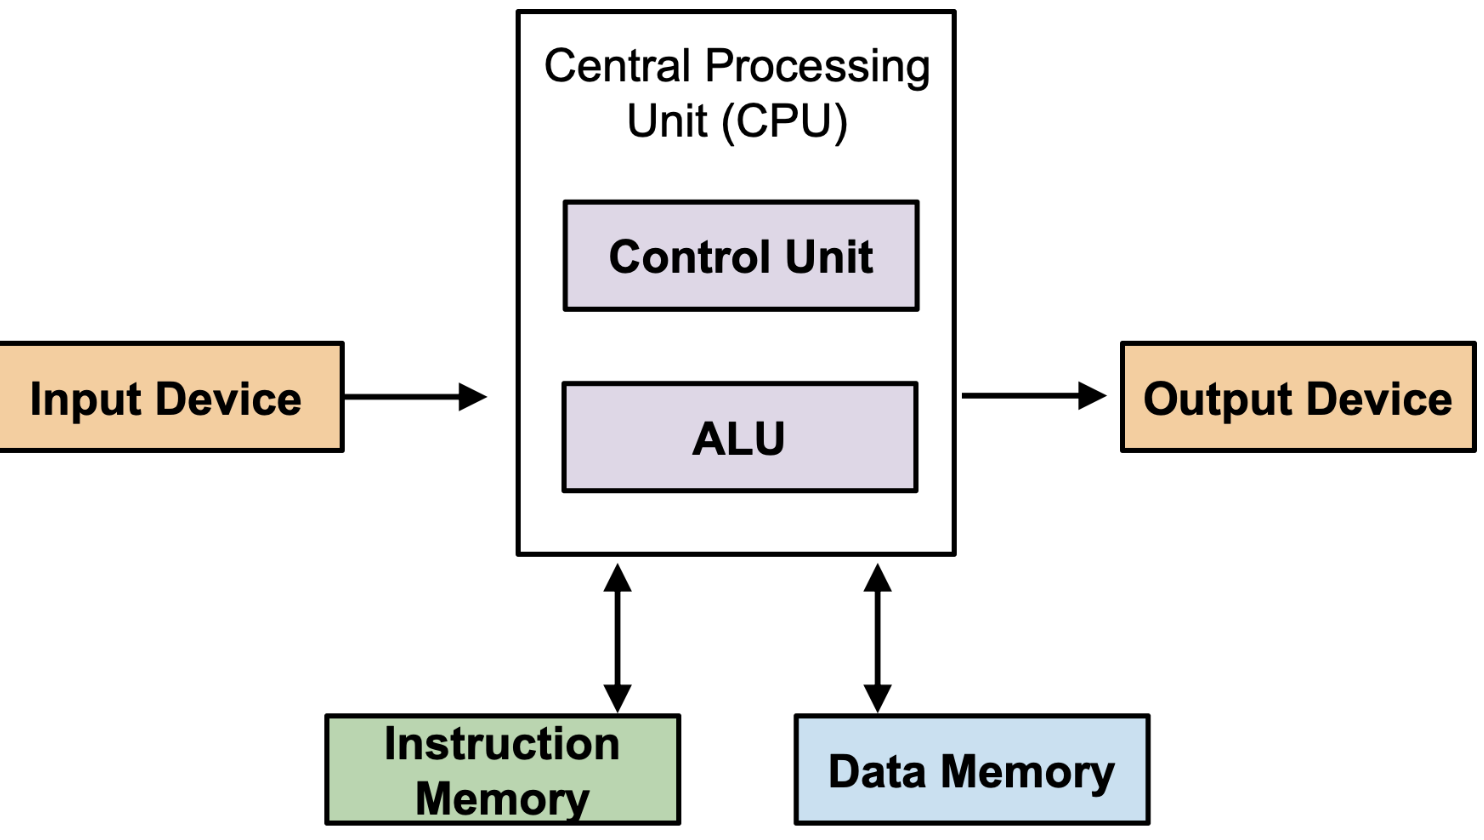
\includegraphics[scale=0.17]{harvard-architecture}
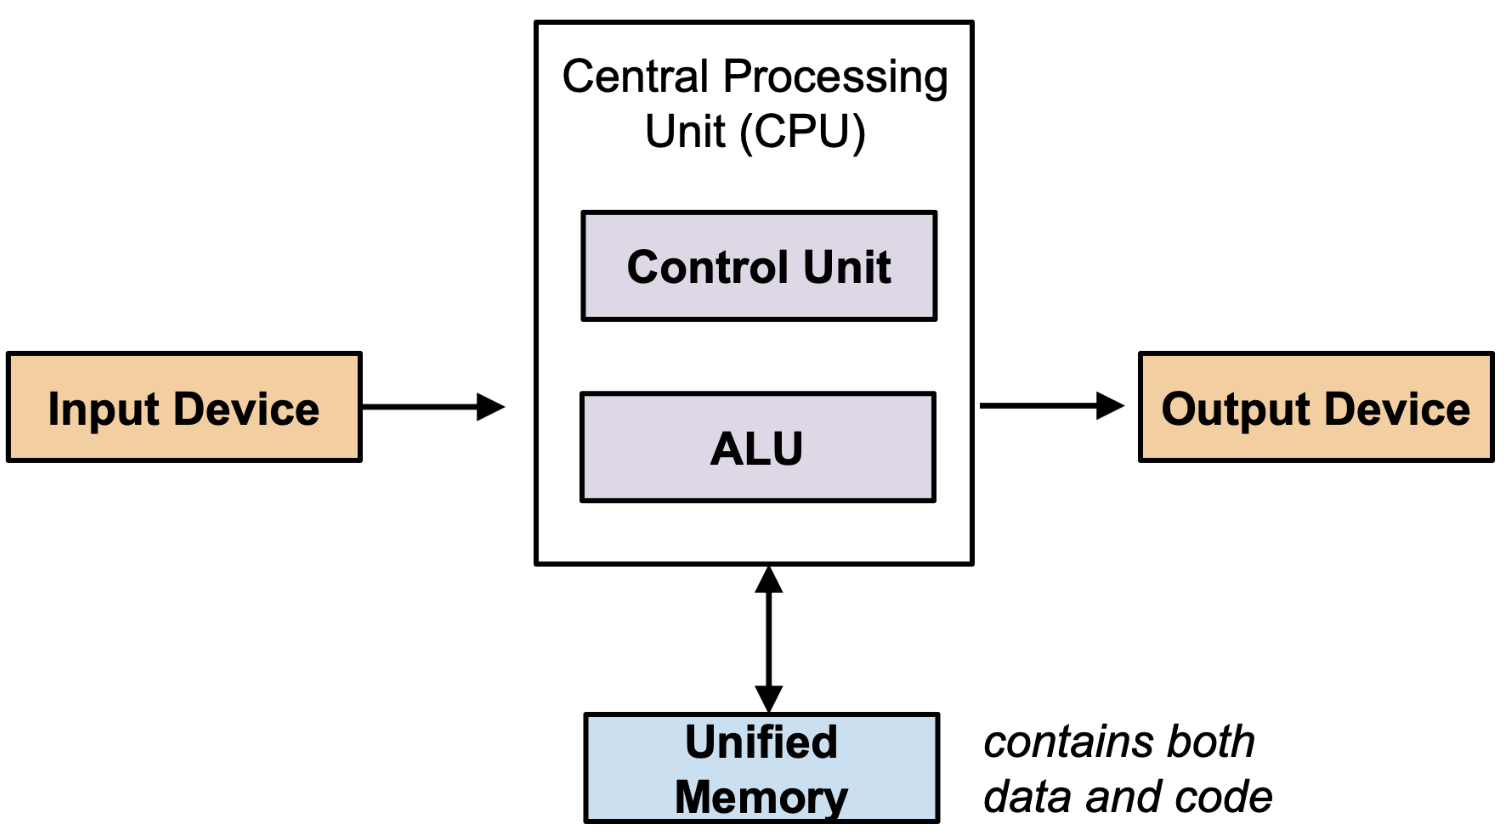
\includegraphics[scale=0.17]{von-neumann}

\begin{description}
	\item[Difference]{Separate vs common storage pathway for code and data}
\end{description}
Why do we need OS?
\begin{itemize}
	\item Should not have bugs
	\item Treat process as malicious
\end{itemize}

\subsection{Mainframe}
Old analog "computers" using physical cards for programming
\subsubsection{Improvements}
\begin{itemize}
	\item Problem: Batch processing inefficient
	\item Solution: Multiprogramming
	\begin{itemize}
		\item Loading multiple jobs that runs while other jobs using I/O
		\item Overlapping computation with I/O
	\end{itemize}
	\item Problem: Only one user 
	\item Solution: Time sharing OS
	\begin{itemize}
		\item Multiple concurrent users using terminals
		\item User job scheduling 
		\item Memory management
		\item \keyword{Hardware virtualization}{Each program executes as if it had all resources}
	\end{itemize}
\end{itemize}


\subsection{Motivation}
\begin{enumerate}
	\item Abstraction
	\begin{itemize}
		\item Hide low level details and present common, high-level functionality to users
	\end{itemize}
	\item Resource allocation
	\begin{itemize}
		\item Allow concurrent usage of resource and execute programs simultaneously
		\item Arbitrate conflicting request fairly and efficiently
	\end{itemize}
	\item Control programs
	\begin{itemize}
		\item Restrict resource allocation
		\item Security, protection and error prevention (Defensive)
		\item Ensure proper use of device
	\end{itemize}
\end{enumerate}
\subsubsection{Advantage}
\begin{itemize}
	\item Portable and flexible
	\item Use computer resources efficiently
\end{itemize}
\subsubsection{Disadvantage}
\begin{itemize}
	\item Significant overhead
\end{itemize}

\subsubsection{OS vs User Program}
Similarities
\begin{itemize}
	\item Both softwares
\end{itemize}
Difference
\begin{itemize}
	\item OS runs in \keyword{kernel mode}{Access to all hardware resources}
	\item User programs run in \keyword{User mode}{Limited access}
		\columnbreak
	\item User programs use syscalls to communicate with OS for hardware processes
	\item User - Full virtual address space for code but cannot write outside of virtual address space
	\item Kernel - All code share same address space
\end{itemize}
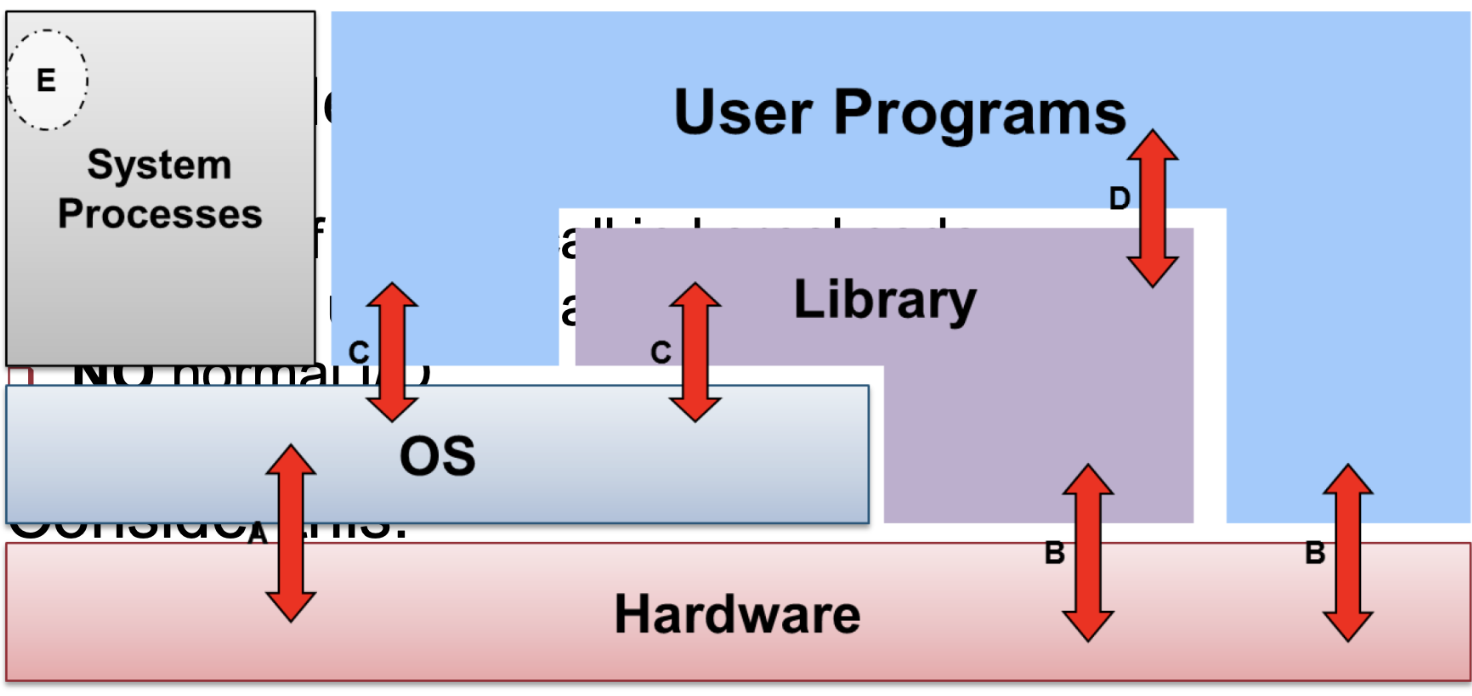
\includegraphics[scale=0.22]{os-interaction}
\begin{description}
	\item[A]{OS executes machine instructions}
	\item[B]{Normal machine instructions executed}
	\item[C]{Calling OS using \textbf{syscall interface}}
	\item[D]{User programs call library code}
	\item[E]{System processes providing high level services}
\end{description}
Why OS dont occupy entire hardware layer
\begin{itemize}
	\item Slow to have all operations pass through intermediary
	\item User programs can have direct interaction with hardware (eg. Arithmetic) during low risk operations
\end{itemize}

\subsection{OS structure}
\subsubsection{Monolithic OS}
\begin{itemize}
	\item One big kernel program
	\item Well understood and has good performance
	\item Highly \keyword{coupled}{internal structure interconnected that unintentionally affect each other}
\end{itemize}
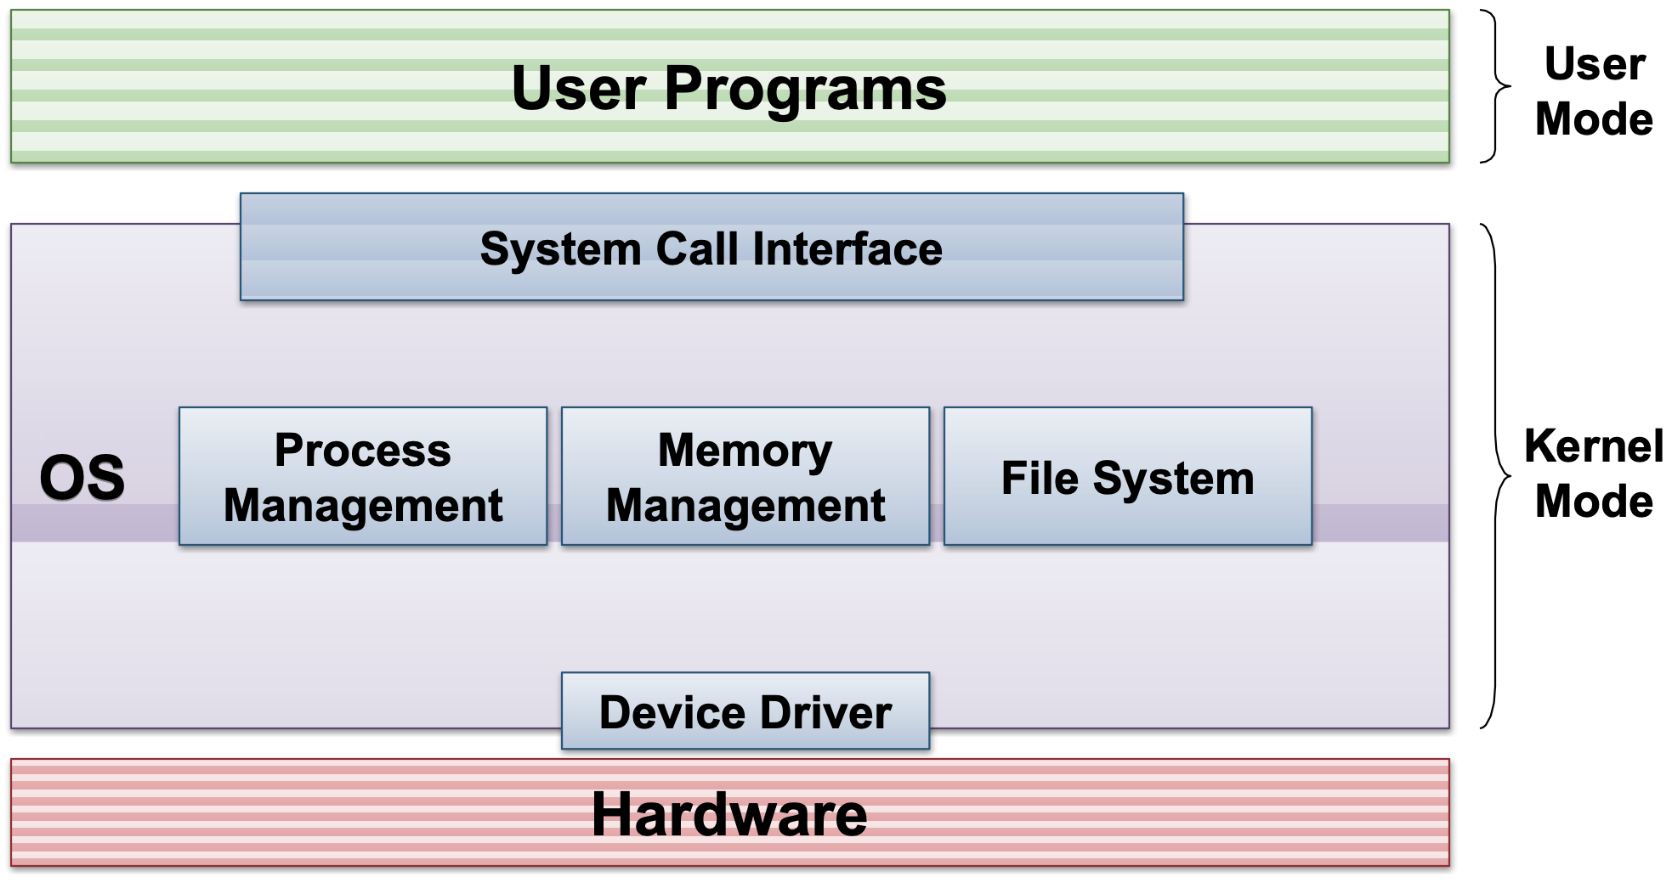
\includegraphics[scale=0.16]{monolithic-os}
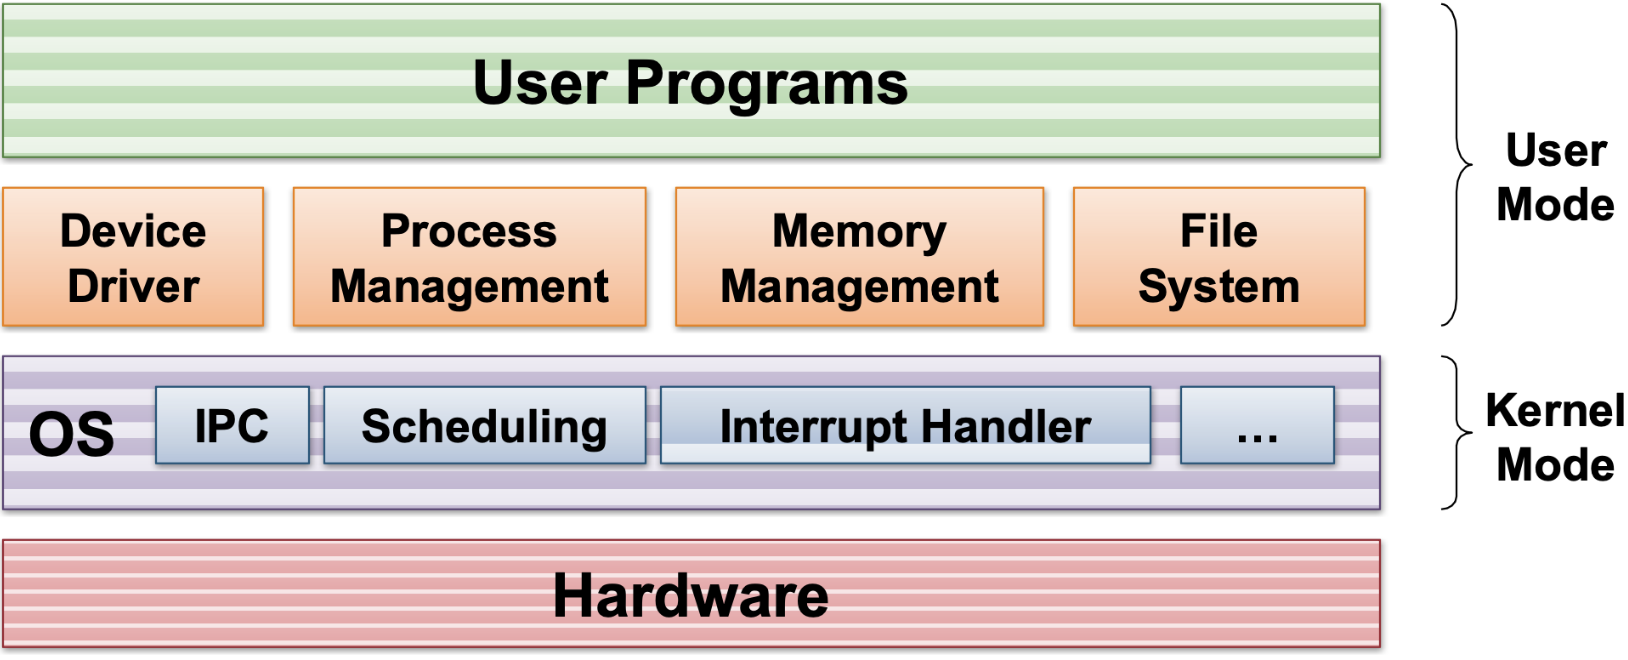
\includegraphics[scale=0.18]{microkernel-os}

\subsubsection{Microkernel}
\begin{itemize}
	\item Small clean
	\item Basic and essential facilities
	\item IPC communication OR run external programs outside OS
	\item Robust and more \keyword{modular}{Extendible and maintainable}
	\item Better isolation btw kernel and services
	\item Lower performance
	\item Unix is monolithic kernel, Windows is hybrid 
\end{itemize}
\subsection{Virtual Machines}
\begin{itemize}
	\item Software emulation of hardware
	\item Virtualization of underlying hardware to run additional operating systems concurrently
\end{itemize}
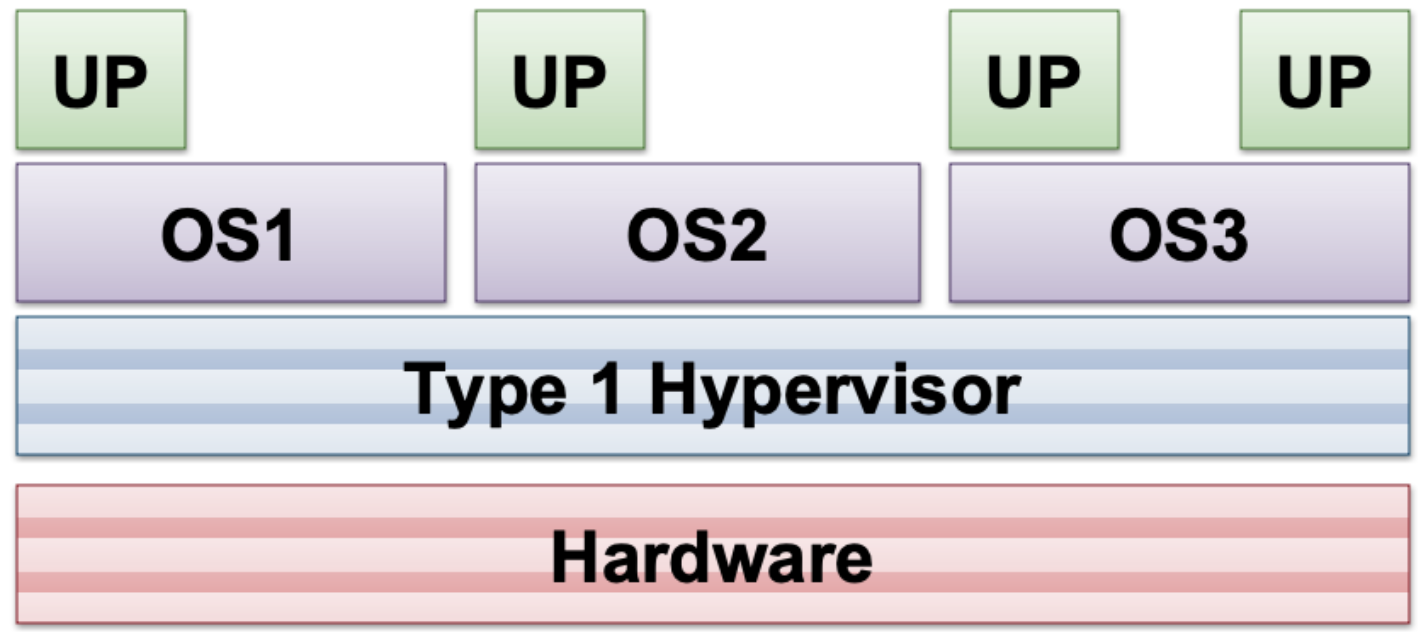
\includegraphics[scale=0.2]{type-1-hypervisor}
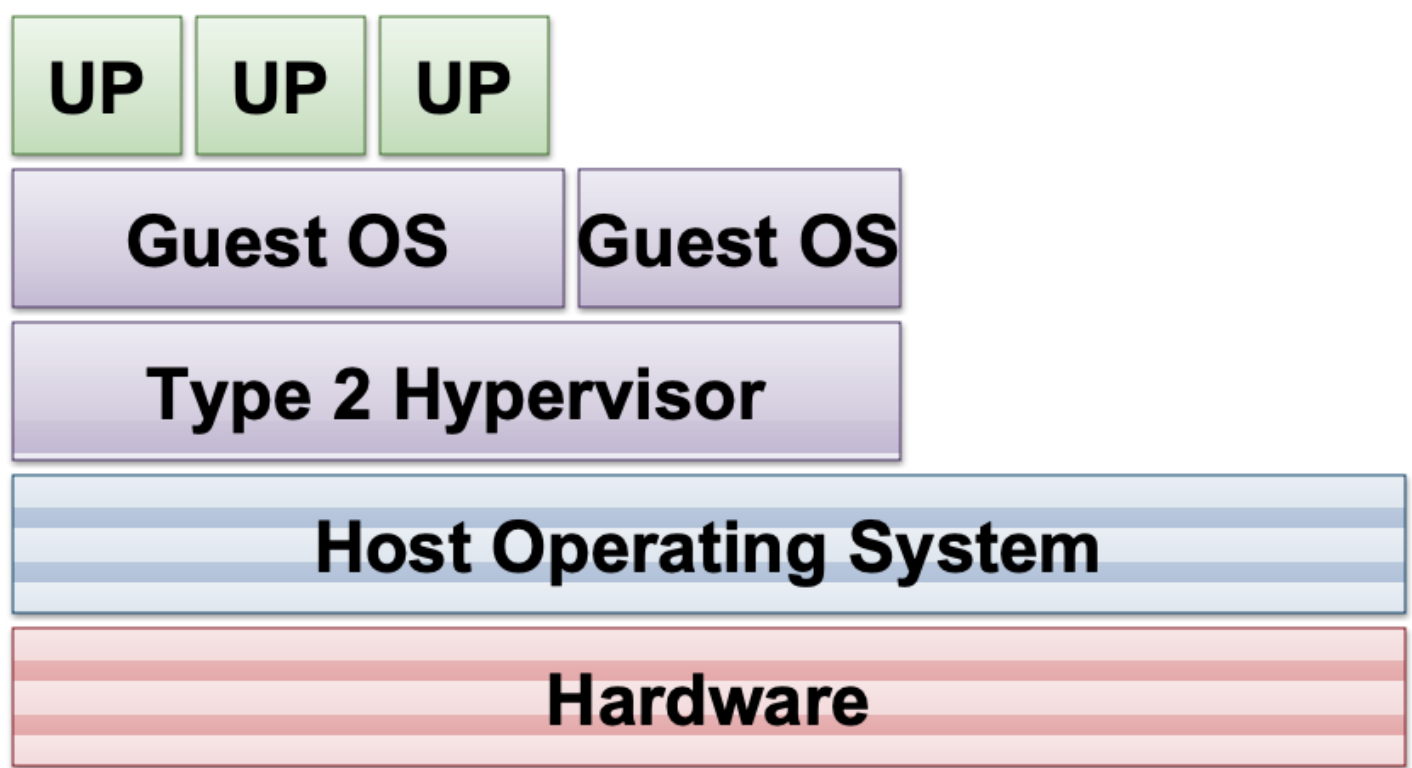
\includegraphics[scale=0.2]{type-2-hypervisor}

%--------------------------------------------------------------------------------------------------------------------

\section{02. Process abstraction}
\subsubsection{Program vs process}
\begin{itemize}
	\item Program is set of instructions to complete a certain task stored in secondary memory of computer
	\item Process is instance of program that is currently executed
	\begin{itemize}
		\item Share the heap with the process but differ in stack
	\end{itemize}
\end{itemize}
\subsection{Motivation}
\begin{itemize}
	\item Allow concurrent usage of hardware
	\item Multiple programs sharing the same processors/IO
\end{itemize}
\subsection{Computer organisation}
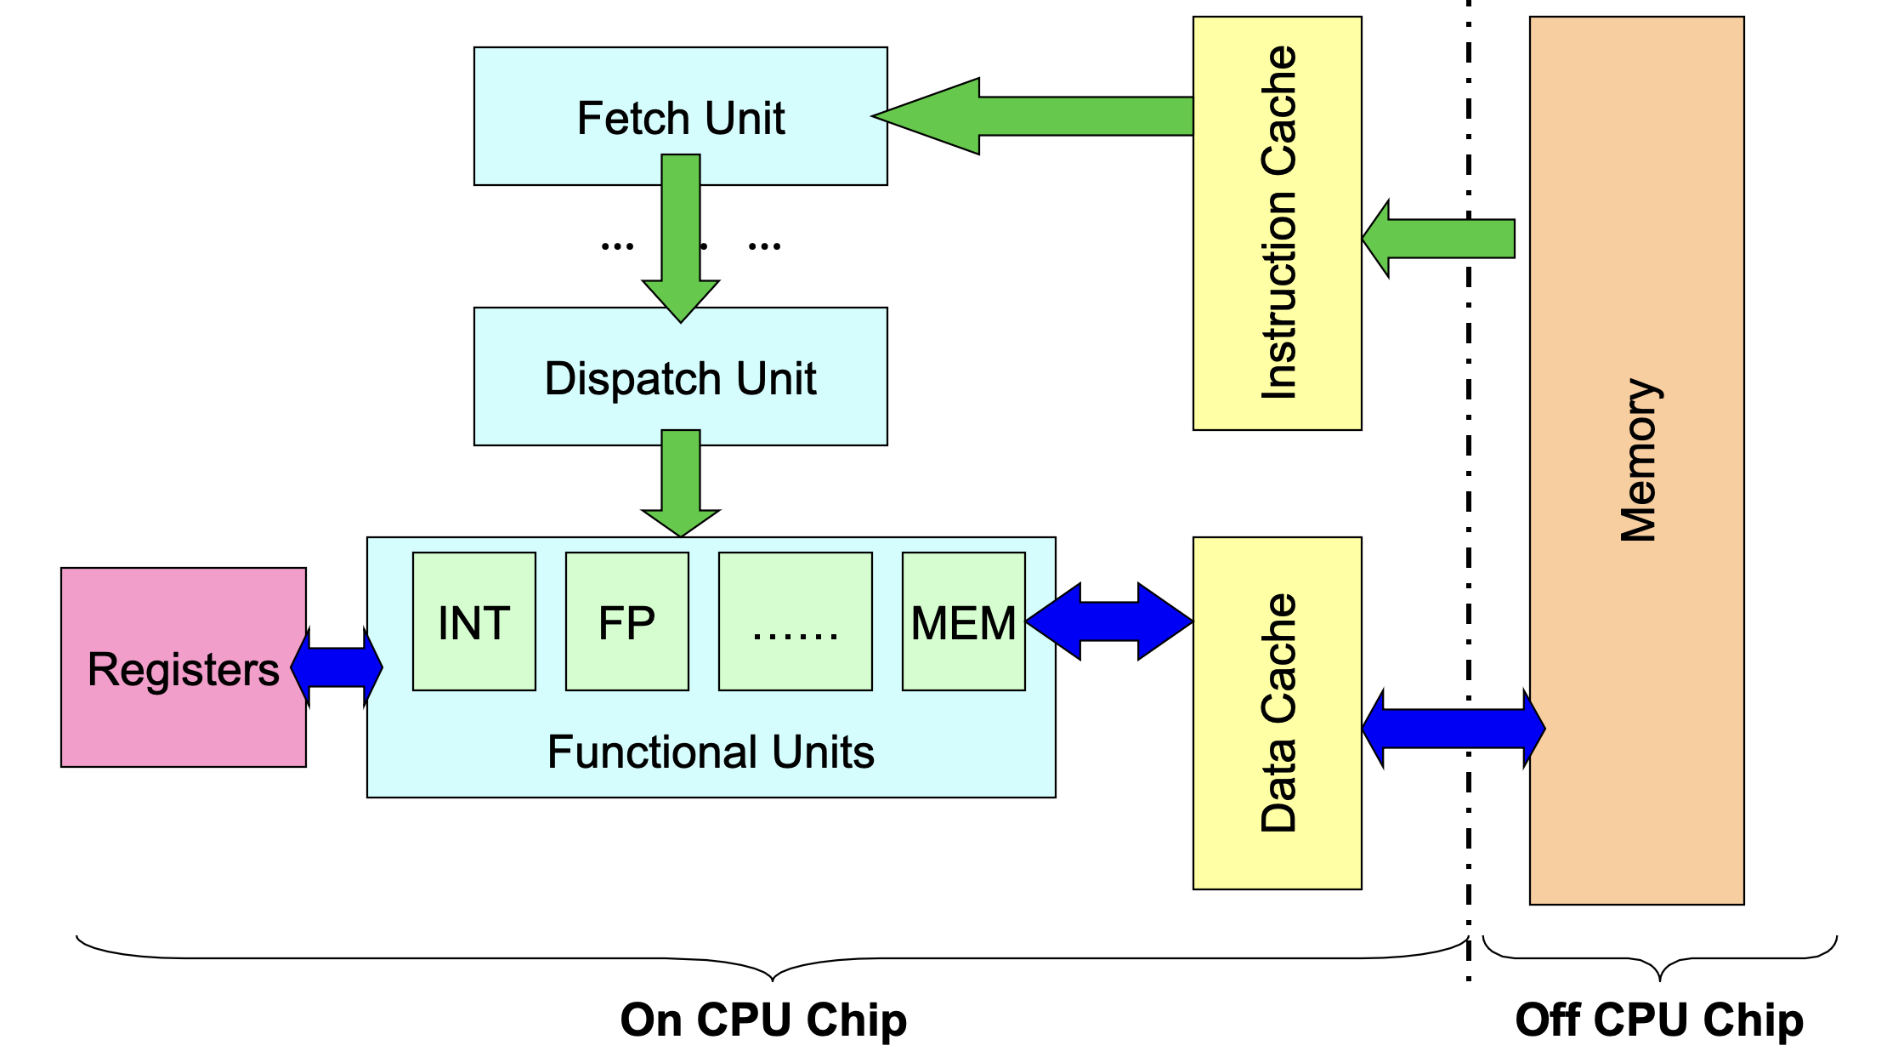
\includegraphics[scale=0.23]{computer-organisation}
\subsubsection{Memory}
\begin{itemize}
	\item Storage for instruction and data
	\item Managed by the OS
	\item Normally accessed via load/store instructions
\end{itemize}
\subsubsection{Cache}
\begin{itemize}
	\item Fast and invisible to software
	\item Duplicate part of the memory for faster access
	\item Usually split into instruction and data cache
\end{itemize}
\subsubsection{Fetch}
\begin{itemize}
	\item Load instructions from memory
	\item Location indicated by \textbf{Program Counter}
\end{itemize}
\subsubsection{Functional units}
\begin{itemize}
	\item Carry out instruction execution
	\item Dedicated to specific instruction type
\end{itemize}
\subsubsection{Registers}
\begin{itemize}
	\item Internal storage for fastest access speed
\end{itemize}
\subsection{Information needed}
\begin{itemize}
	\item Memory context
	\begin{itemize}
		\item Code, data
	\end{itemize}
	\item Hardware context
	\begin{itemize}
		\item Register, PC value, frame pointer
	\end{itemize}
	\item OS context
	\begin{itemize}
		\item Process properties, resource used, files
	\end{itemize}
\end{itemize}
\subsection{Function calls}
Suppose a function f() calls g()
\begin{itemize}
	\item f is caller and g is callee
\end{itemize}
Steps of control flow
\columnbreak
\begin{enumerate}
	\item Setup parameters
	\item Trf ctrl to callee
	\item Setup local var
	\begin{itemize}
		\item Remember the initial variables especially if registers are to be reverted back when jumping back to caller
		\item Callee does not know the registers callers used, so prevent accidental overwrite of content to registers caller use
	\end{itemize}
	\item Store any results
	\item Return ctrl to caller
\end{enumerate}
\subsubsection{Issues}
Control Flow
\begin{itemize}
	\item Need to jump to functional body when callee called
	\item Need to resume to next instruction in caller after done
\end{itemize}
Data storage
\begin{itemize}
	\item Need to pass parameters to function
	\item Need to capture return result
	\item May have local variables
\end{itemize}
Additional
\begin{itemize}
	\item May lead to overriding of data in caller by callee (interference)
	\item Calling g() multiple times may lead to insufficient space and overriding
\end{itemize}


\subsection{Stack memory}
Memory to store function invocation and control flow\\
\keyword{Stack Pointer}{Indicates the first free location in the stack region}\\
\keyword{Frame Pointer}{Points to the frame and is used for traversing around the stack easily}\\
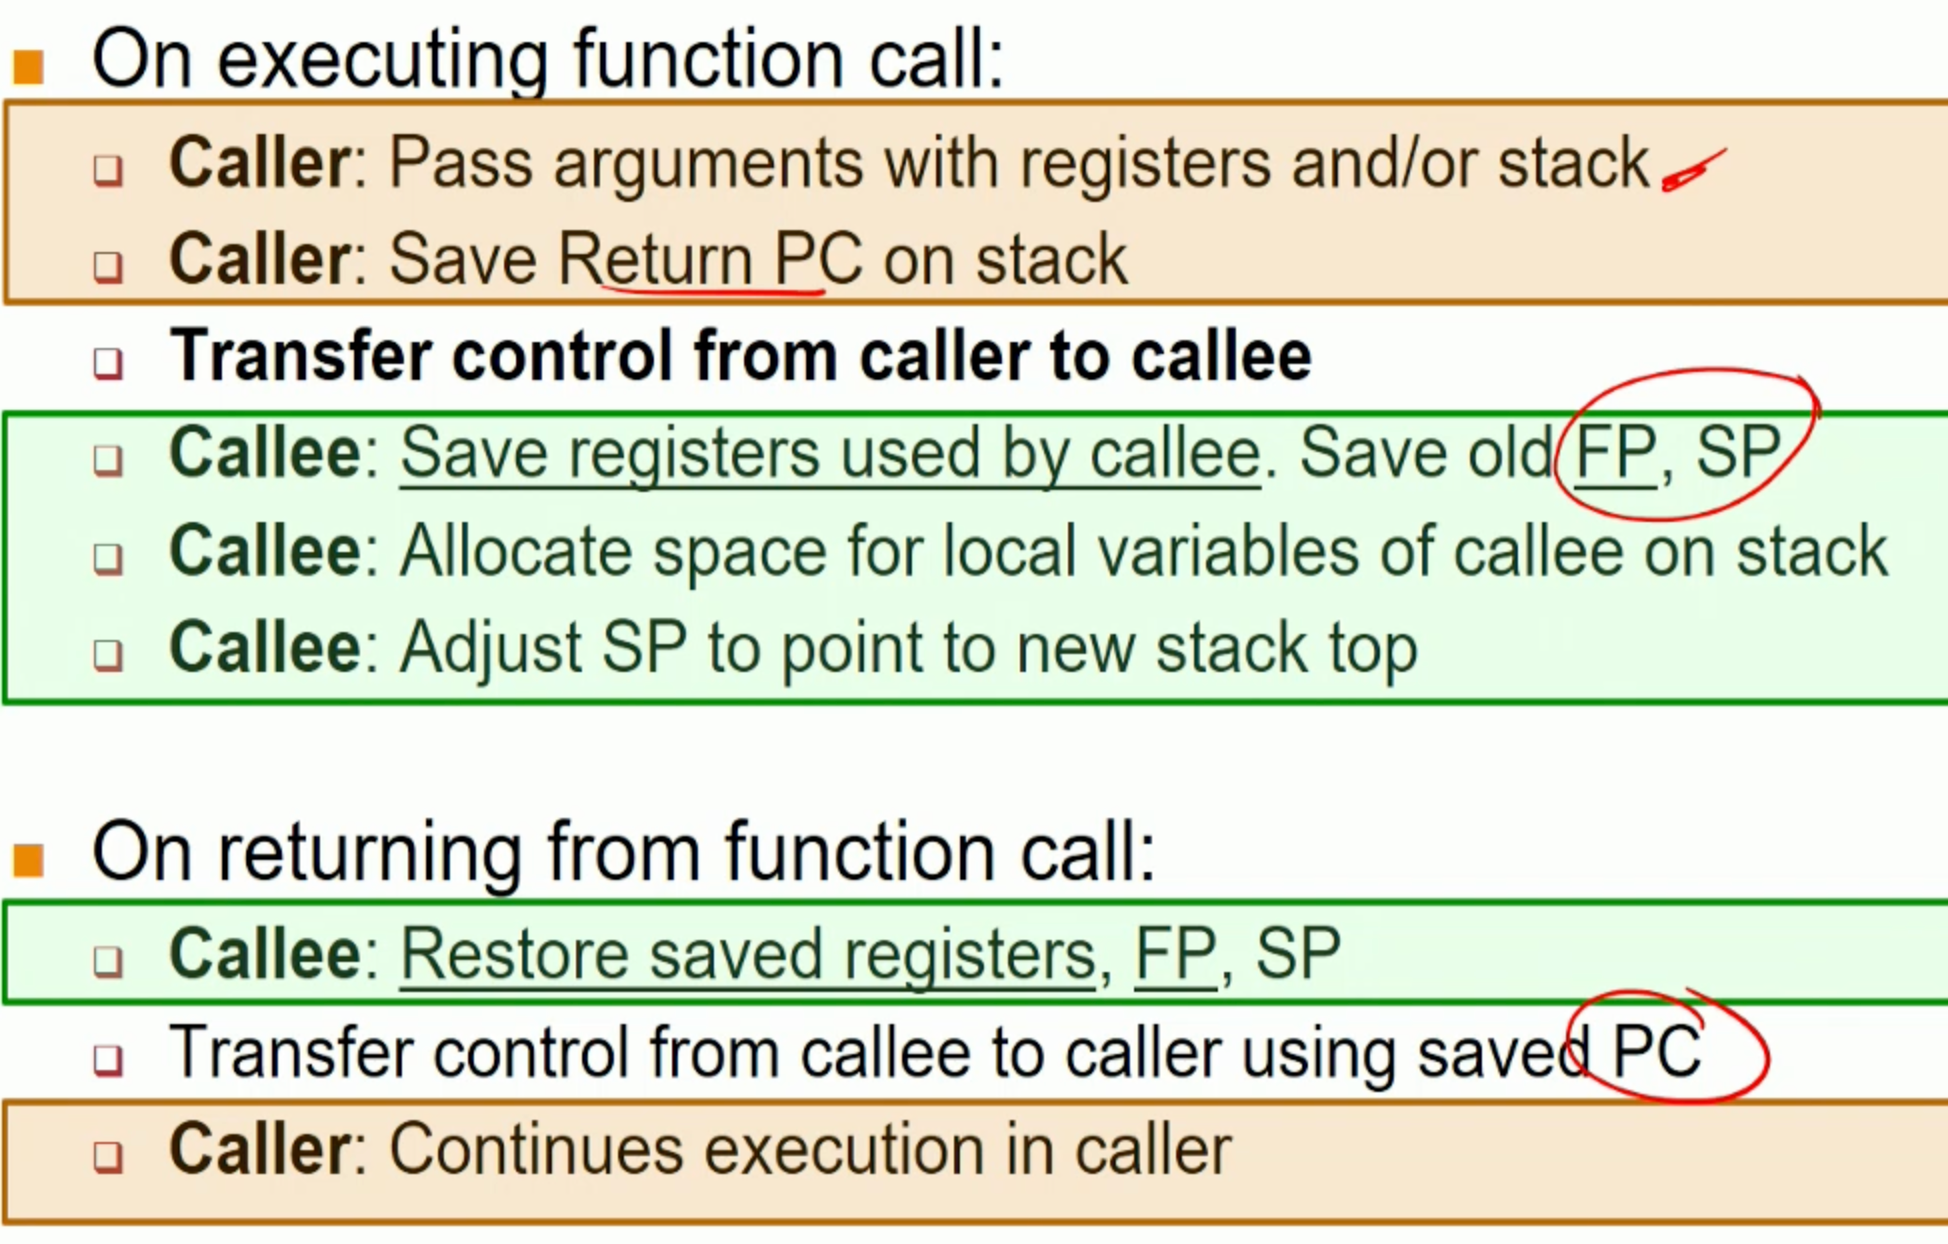
\includegraphics[scale=0.08]{stack-frame}
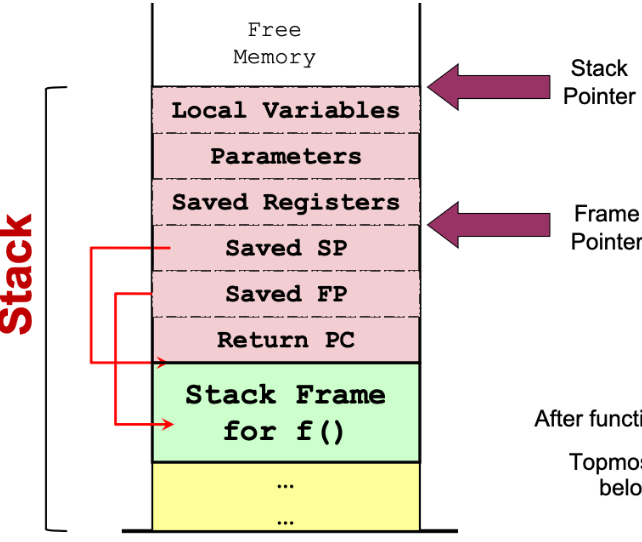
\includegraphics[scale=0.2]{stack-frame-diagram}\\
Information needed for function invocation - Stack frame
\begin{itemize}
	\item Return address of caller
	\item Arguments for the function
	\item Local variables
	\item Stack and frame pointer of caller
	\item GPR values (register spilling)
\end{itemize}
Callee stack frame will be on top of the caller


\subsection{Dynamic memory (Heap)}
Memory that the program/user specifies manually (eg. malloc, new)\\
Problems:
\begin{itemize}
	\item Allocated only at runtime
	\begin{itemize}
		\item Size not known at program compilation time
		\item Cannot specify a region in data 
	\end{itemize}
	\item No definite deallocation timing
	\begin{itemize}
		\item Must be freed explicitly by the program
		\item Cannot place in stack region
	\end{itemize}
\end{itemize}
Solution:\\
Add Heap region for dynamic allocation\\
\begin{itemize}
	\item BUT: Generates holes btw data due to variable deallocation timing
\end{itemize}
\subsection{Stack vs Heap}
\begin{itemize}
	\item Objects are stored in heap and stack stores references to it
	\columnbreak
	\item Objects in heap are globally accessible 
	\item Data are primitive variables eg. int, char.. even when not initialized
\end{itemize}

%-----------------------------------------------------------------------------------------------------------------------
\subsection{OS context}
\subsubsection{Process identification}
Features:
\begin{itemize}
	\item Distinguish processes from each other (Unique)
	\item Communicated to the hardware
\end{itemize}
\subsubsection{Process state}
\begin{description}
	\item[New]{New process that may still be under initialization (not schedulable)}
	\item[Ready]
	\item[Running]{Executed on CPU}
	\item[Blocked]{Sleeping/waiting for event - cannot execute until event available}
	\item[Terminated]{Finished execution and requires OS cleanup}
\end{description}
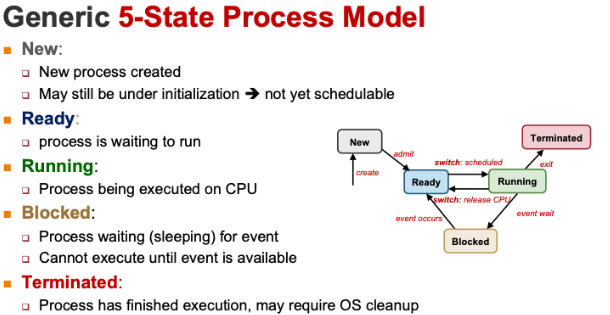
\includegraphics[scale=0.2]{process-model}
\subsection{Process control block (PCB)}
Table representing all processes containing entire execution context 
\begin{itemize}	
	\item Maintained by OS in OS memory for every process
	\item PC, FP, SP and other GPR (only updated when swapped out)
	\item Memory region info (Text, data, heap and stack)
	\begin{itemize}
		\item It is a "point" to real memory space \textbf{NOT actual memory space used by process}
	\end{itemize}
	\item PID, privileges, process state
	\item Pointer to parent process
\end{itemize}
\subsubsection{Context switching}
\begin{enumerate}
	\item Interrupt or syscalls
	\item Save state of old process into PCB
	\item Reload state of new process from PCB
\end{enumerate}
\begin{itemize}
	\item Only saves the state of CPU registers
	\item Involves a change to kernel mode and back
\end{itemize}
\subsection{Exceptions and interrupts}
Exceptions
\begin{itemize}
	\item Synchronous (due to program execution)
	\item Machine level instructions arise errors
	\item Exception handler executed automatically in software (can be handled by programmer)
	\item Handled by OS which sends a signal to application to implement try-catch mechanism
\end{itemize}
Interrupts
\begin{itemize}
	\item Asynchronous (Can happen anytime)
	\item External events that cause execution to fail (hardware related errors)
	\item Program execution suspended and \textbf{interrupt handler} executed automatically
\end{itemize}
\subsubsection{Instruction execution}
\begin{enumerate}
	\item Read byte from PC and decode instruction
	\item Read 2 bytes to get the address/operands
	\item Perform ALU operations
	\item Store result into destination
	\item Check if any interruptions
\end{enumerate}
Interrupts can happen at anytime, and will remain pending until step 5 where it is handled

\subsubsection{Interruption handling}
\begin{enumerate}
	\item Push PC and status register into hardware
	\item Disable interrupts
	\item Read \keyword{Interrupt Vector Table}{Table where the OS stores address of all interrupt handlers}
	\item Switch to kernel mode
	\item Set PC to handler address and execute the instructions
\end{enumerate}
\begin{itemize}
	\item OS populates the IVT table with address of interrupt routines
	\item Hardware reads IVT to locate the handler
\end{itemize}
\subsection{System calls}
\keyword{Application Program Interface}{Provides way of calling facilities/services in kernel}\\
Synchronous function only done in kernel mode providing system services\\
Typically more expensive than library calls due to context switching\\
OS dependent anc cannot be avoided by any application
\subsubsection{Functions}
\begin{description}
	\item[Process control]{Direct processes like creating, terminating or synchronisation}
	\item[File/device manipulation]
	\item[Information maintenance]{Get system data, time, etc}
	\item[Communication]{Create, delete connections and send/receive messages}
\end{description}
\subsubsection{Method (Programming language specific)}
\begin{itemize}
	\item Library version with the same name and same arguments 
	\item User friendly library version
	\item Using func $long~syscall(long~number);$
\end{itemize}
\subsubsection{Mechanism}
\begin{enumerate}
	\item User invoke library call
	\item Place call number in the designated location
	\item Library call executes a special instruction (\textbf{TRAP/syscall}) to change user to kernel mode
	\item (in kernel) syscall handler is determined (by a \textbf{dispatcher})
	\item syscall handler is executed
	\item Syscall handler ends and control returned to the library call
	\item Return to user mode and continue normal function mechanism
\end{enumerate}


%--------------------------------------------------------------------------------------------------------------------
\section{03. Process abstraction in Unix}
Process information
\begin{description}
	\item[Pid]
	\item[Proc state]{Running, sleeping, stopped, zombie}
	\item[Parent pid]
	\item[Cumulative CPU time]{For scheduling}
\end{description}

\subsection{fork() syscall}
Process creation
\begin{description}
	\item[Package]{unistd.h and sys/types.h}
	\item[return]{PID of newly created process(parent) and 0 (child process)}
	\item[handler]{Code is stored in the OS memory region}
\end{description}
\subsubsection{Behaviour}
\begin{itemize}
	\item Creates a child process
	\begin{itemize}
		\item \textbf{Copy} data of parent (Independent memory space)
		\item Unless explicitly modifying value at address, parent and child variables are distinct
		\item Sane code, same address space
		\item Differs by pid, ppid and fork() return value
	\end{itemize}
\end{itemize}

\subsubsection{Implementation}
Clone the parent process 
\begin{enumerate}
	\item Create address space of child process
	\item allocate new pid to child and pass to parent
	\item Create kernel process data structures
	\item Copy kernel environment of parent process
	\item Initialize child process context (pid, ppid, cpu\_time = 0)
	\item Copy memory regions from parent
	\begin{itemize}
		\item Very expensive operation
		\item Code, data, stack
	\end{itemize}
	\item Acquire shared resources
	\item Initialize hardware context for child process (copy parent registers)
\end{enumerate}

Problem: Memcopy is very expensive operation\\
Solution: Copy on write
\begin{itemize}
	\item Only duplicate a memory location when it is written to
\end{itemize}

\subsection{exec(@param)}
Replace current executing process image
\begin{itemize}
	\item Code and data replaced
	\item PID/PPID intact
	\item If fail, program just continues to run the next instruction
\end{itemize}
Format
\begin{description}
	\item[param]{char *path, char *arg0...}
	\begin{itemize}
		\item Note that last term MUST be \textbf{NULL} indicating end of argument list
	\end{itemize}
	\item[header]{unistd.h}
\end{description}

\subsection{exit(status)}
\begin{description}
	\item[return]{Does not return anything}
	\item[param]{int status - returned to the wait call}
\end{description}
\begin{itemize}
	\item Most system resource used by process are released on exit
	\item return from main() implicitly calls exit(0)
	\item Basic processes are not releasable
	\begin{itemize}
		\item Pid and status
		\item Process accounting info
	\end{itemize}
\end{itemize}

\subsection{wait(\&status)}
Parent child synchronisation
\begin{description}
	\item[param]{\&status - address to put return value}
	\item[header]{sys/types.h and sys/wait.h}
	\item[return]{pid of terminated process}
\end{description}
\begin{itemize}
	\item Call is blocking - suspend operation until at least one child terminates
	\item Cleans up remainder of child system resources (PID, status)
	\item waitpid - used for waiting for specific child process
\end{itemize}

\subsection{Orphan and zombie process}
\keyword{Zombie}{\textbf{All} processes that has exited but parent did not call wait}\\
\begin{itemize}
	\item Processes can be cleared by rebooting system
\end{itemize}
\keyword{Orphan}{Child process whose parent has been terminated}
\begin{itemize}
	\item Parenthood will be propagated up to init which may use wait() to clean up
	\item Can be manually terminated from interpreter or reboot system
\end{itemize}


%--------------------------------------------------------------------------------------------------------------------
\section{04. Inter Process Communication}

\subsection{Mechanism}
\begin{itemize}
	\item Shared memory
	\item Message passing
	\begin{itemize}
		\item Pipes
		\item Signal
	\end{itemize}
\end{itemize}

\subsection{Shared memory}
Communication through read/write to shared memory\\
Advantages
\begin{description}
	\item[Efficient]{Only require OS to setup shared region once}
	\item[Ease of use]{Simple reads and write to memory}
	\begin{itemize}
		\item Implicit communication
		\item Can store any type of information
	\end{itemize}
\end{description}
Disadvantages
\begin{description}
	\item[Limited to single machines]{Less efficient over different system}
	\item[Need Sync]{Might have data races without synchronisation}
\end{description}
\keyword{Race condition}{System behaviour is dependent on the context/interleaving of process $\rightarrow$ unpredictable outcome}
\subsubsection{Steps}
\begin{enumerate}
	\item Create/locate a shared memory region M
	\item Attach M to process memory space
	\item Read from/write to M
	\item Detach M from memory space after use
	\item Destroy M
	\begin{itemize}
		\item Only one process need to do this
		\item Can only destroy if M is not attached to any process
	\end{itemize}
\end{enumerate}

\subsection{Message Passing}
Explicit communication through exchange of message
\begin{description}
	\item[Naming]{Have to identify the parties in the communication}
	\item[Synchronisation]{Behaviour of sending/receiving operations}
\end{description}
\begin{itemize}
	\item Messages have to be stored in kernel memory space
	\item All sending/receiving operations have to be done through syscalls
\end{itemize}
\subsubsection{Direct communication}
Sender/receiver explicitly name parties in communication
\begin{itemize}
	\item One link per pair of communicating processes
	\item Need to know identity of other party
\end{itemize}

\subsubsection{Indirect communication}
Message storage (\textbf{Mailbox/Port})
\begin{itemize}
	\item Can be shared among a number of processes
\end{itemize}

\subsubsection{Synchronisation behaviour}
Blocking
\begin{itemize}
	\item send and receive is blocked until a message has received/sent (other party is ready)
\end{itemize}
Non-blocking (asynchronous)
\begin{itemize}
	\item execute immediately and sends information to somebody OR returns empty handed
\end{itemize}
Typically, receive is synchronous and send is asynchronous\\
BUT send just buffers the message and only sends the message when the receiver is receiving (no loss)\\
Message buffers
\begin{itemize}
	\item Under OS control 
	\item Decouples sender and receiver -\> less sensitive to variation in execution
	\item Mailbox capacity declaration in advance
\end{itemize}
\textbf{Rendezvous}
\begin{itemize}
	\item Synchronous message passing 
	\item Sender is blocked until receiver sends matching receive
	\item No buffering needed
\end{itemize}

\subsubsection{Pros}
\begin{itemize}
	\item Applicable beyond a single machine
	\item \keyword{Portable}{Easily implemented on many platforms and processing environments}
	\item Easier synchronisation
	\begin{itemize}
		\item Implicit via send/receive behaviour
		\item Communication and synchronisation is done simultaneously
	\end{itemize}
\end{itemize}
\subsubsection{Cons}
\begin{description}
	\item[Inefficient]{Usually requires OS intervention every operation}
	\item[Difficult to use]{Requires information packing into specific format}
\end{description}

\subsection{Unix Pipes}
3 different communication channels to user
\begin{enumerate}
	\item stdin - standard in bounded to keyboard input
	\item stderr - used for error messages
	\item stdout - linked to screen
\end{enumerate}
$"|"$ symbol for linking input/output channels of each process to each other\\
Create communication channel with 2 ends (one reading, one writing)
\begin{itemize}
	\item Producer-consumer relationship
	\item Like anonymous file reading information FIFO
\end{itemize}
\subsubsection{Synchronisation}
\begin{itemize}
	\item Circular bounded byte buffer with implicit synchronization
	\item Writer wait when buffer is full
	\item Reader wait when buffer is empty
	\item Unidirectional (one write one read exclusively) vs bidirectional (any end for reading and writing)
\end{itemize}
\subsubsection{pipe(@param)}
\begin{description}
	\item[param]{array of file descriptors}
	\item[return]{0 for success, != for errors}
\end{description}
\subsection{Unix signals}
Asynchronous notification about an event sent to process/threads
\begin{itemize}
	\item Handle signal via default or user defined/supplied handlers(not all signals)
	\item Can only call async safe functions within handler (signal/wait cannot be called in POSIX)
	\item eg. Kill, stop, continue, error
\end{itemize}
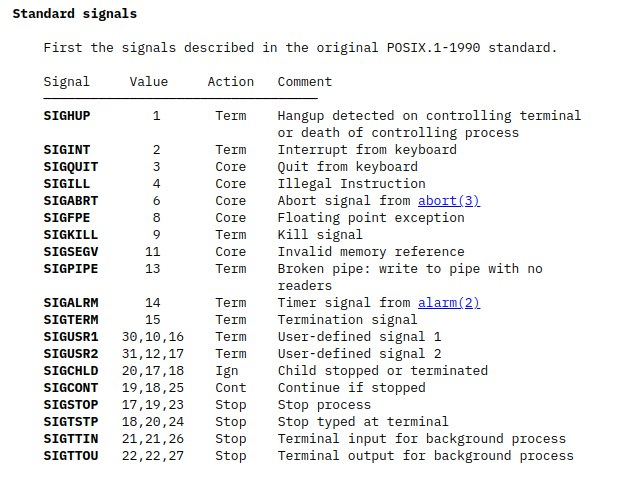
\includegraphics[scale=0.38]{common-signals}

%--------------------------------------------------------------------------------------------------------------------

\section{05.Process scheduling}
Concurrency
\begin{itemize}
	\item Multiple process progress at the same time
	\item Virtual parallelism (threading, context switching)
	\item Physical parallelism (multicore, multi CPU)
\end{itemize}

\subsection{Scheduling}
More ready processes vs limited CPU
\begin{itemize}
	\item Each process diff CPU usage
	\item \keyword{Scheduling algorithms}{Deciding the process to run based on environment and process behaviour}
	\item Processes have phases of io-bound and cpu intensive activities
\end{itemize}
Processing environment (sorted by increasing user interaction and response times):
\begin{enumerate}
	\item Batch
	\item Interactive
	\item Real time
\end{enumerate}
\subsection{Objectives}
\begin{description}
	\item[Fairness]{Should get fair share of CPU time n prevent \keyword{starvation}{processes never have access to CPU}}
	\item[Utilization]{Hardware is used all the time}
\end{description}
\keyword{non-preemptive}{Process gives up resources voluntarily}
\keyword{preemptive}{Process given a fixed quota to run and is suspended for other processes}
\subsection{Timeline}
\begin{enumerate}
	\item Scheduler is triggered (OS take over)
	\item Context switching can happen and current process information stored and placed back in queue
	\item Pick process to run using algorithm and setup its context
\end{enumerate}

\subsection{Batch}
Non-preemptive used dominantly cos minimal user interaction needed
\subsubsection{Objectives} 
\begin{description}
	\item[Turnaround time]{Total time till finish running \textbf{including waiting} (finish time - arrival time)}
	\item[Throughput]{Rate of task completion}
	\item[Makespan]{Total time to complete \textbf{ALL} tasks}
	\item[CPU utilization]{Percentage of \textbf{time} CPU is used}
\end{description}
\subsubsection{Algorithms}
\begin{enumerate}
	\item First Come First Serve (FCFS)
	\begin{itemize}
		\item Scheduled using FIFO queue based on arrival time (bad turnaround time)
		\item Guarantee no starvation - number of tasks in front of task is strictly decreasing
		\item Reordering can reduce waiting time 
		\item \keyword{Convoy Effect}{Not all hardware resources are used concurrently because a process blocks it}
	\end{itemize}
	\item Shortest Job First (SJF)
	\begin{itemize}
		\item Choose tasks with smallest total CPU time
		\item Estimate CPU time for tasks in advance using the previous CPU-bound phases
		\item $Estimated_{n+1} = \alpha Actual_{n} + (1-\alpha) Predicted_{n}$
		\item Starvation is possible as long tasks end up continuously waiting
	\end{itemize}
	\item Shortest Remaining Time (SRT)
\end{enumerate}

\subsection{Interactive system}
\subsubsection{Objectives}
\begin{description}
	\item[Response time]{Time between request and response by system}
	\item[Predictability]{Decreased variation in response time}
	\item[Premptive scheduling]
\end{description}
\begin{itemize}
	\item Periodic scheduler with time interrupts
	\item \keyword{Time quantum}{Execution duration given to a process}
	\begin{itemize}
		\item Constant(regardless whether the process has given up processing halfway) OR Variable(full time quantum given to a process)
	\end{itemize}
\end{itemize}
\subsubsection{Algorithms}
\begin{enumerate}
	\item Round Robin (RR)
	\begin{itemize}
		\item Store tasks in FIFO queue and pick tasks to run until
		\begin{enumerate}
			\item Fixed time slice elapsed
			\item Task gives up CPU voluntarily
			\item Task blocks
		\end{enumerate}
		\item Task placed at end of queue to wait for next turn
		\item Response time guaranteed bounded by num task \* time quantum
		\item Timer interrupt needed
		\item Choice of time quantum duration is important 
		\begin{itemize}
			\item Longer quantum: Better utilization but greater wait time
			\item Shorter quantum: Bigger overhead/ lower utilization but shorter wait time
		\end{itemize}
		\item Poor performance when there are many jobs all exceeding time quantum -\> high overhead from context switching
	\end{itemize}
	\item Priority scheduling
	\begin{itemize}
		\item Assign tasks processes priorities based on impt and select them
		\item Starvation for low priority tasks
		\begin{itemize}
			\item Solution: 
			\item Lower priority every time the process have executed
			\item Give processes a time quantum
		\end{itemize}
		\item \keyword{Priority Inversion}{Lower priority tasks locks the resources used by a higher priority task leading to deadlock OR allowing lower priority tasks to run before}
		\begin{itemize}
			\item Solution:
			\item Temporarily increase priority of tasks that lock resources until it unlocks
			\item Low priority task inherit the priority of high priority tasks which is restored once unlocked
		\end{itemize}
	\end{itemize}
	\item Multi-level Feedback Queue (MLFQ)
	\begin{itemize}
		\item Runs processes with higher priorities but lower priority when the job fully utilise its time quantum
		\item Processes that voluntarily gives up/blocks before time quantum retains its priority
		\item New processes have highest priority
		\item Processes with same priority run in RR
		\item Long CPU processes are starved as its priority becomes very low and cannot complete
		\begin{itemize}
			\item Solution: Occassionally reset tasks to full priority 
		\end{itemize}
		\item Processes can exploit and voluntarily give up to retain its priority
		\begin{itemize}
			\item Solution: Peg priority based on total CPU usage instead 
		\end{itemize}
	\end{itemize}
	\item Lottery scheduling
	\begin{itemize}
		\item Give out tickets to processes for various system resources and randomly pick winners to be granted the resources
		\item \keyword{Responsive}{Newly created processes can immediately join the lottery}
		\item Good control - Process can be assigned quantity of tickets and resources which can be shared among its children/threads
		\item Simple implementation
	\end{itemize}
\end{enumerate}
%--------------------------------------------------------------------------------------------------------------------
\section{06.Synchronisation primitives}
\subsection{Race condition}
\begin{itemize}
	\item Execution of sequential processes should be \keyword{deterministic}{Repeated execution returns the same result}... however,
	\item Process sharing modifiable resources AND execute concurrently by interleaving may cause synchronization problems -\> non deterministic outcomes
	\item Order determines the execution outcome
\end{itemize}

\subsection{Critical section}
Region where unsynchronised access could lead to incorrectly interleaving scenarios\\
Only \textbf{ONE} process should be in the critical section at one time
\subsubsection{Properties}
\begin{description}
	\item[Mutual exclusion/Mutex]{All other processes should be blocked from entering critical section if occupied}
	\item[Progress]{If no process occupying section, waiting process should be granted access}
	\item[Bounded wait]{Upper bound on number of times other processes can enter critical section before a waiting process}
	\item[Independence]{Process not in critical section should not block other process}
\end{description}
\subsubsection{Incorrect synchronization}
\begin{description}
	\item[Deadlock]{All processes blocked}
	\item[Livelock]{Processes keep changing states to avoid deadlock resulting in no progress (Deadlock avoidance mechanism)}
	\item[Starvation]
\end{description}
\subsection{Implementations}
\begin{itemize}
	\item High level language implementation (Peterson Algorithm)
	\begin{itemize}
		\item Busy waiting - Repeatedly tests while-loop condition instead of going into blocked state (Wastes CPU power)
		\item Low level - Error prone and complicated
		\item Not general - cannot extend to allowing multiple access instead of Mutex
	\end{itemize}
\end{itemize}
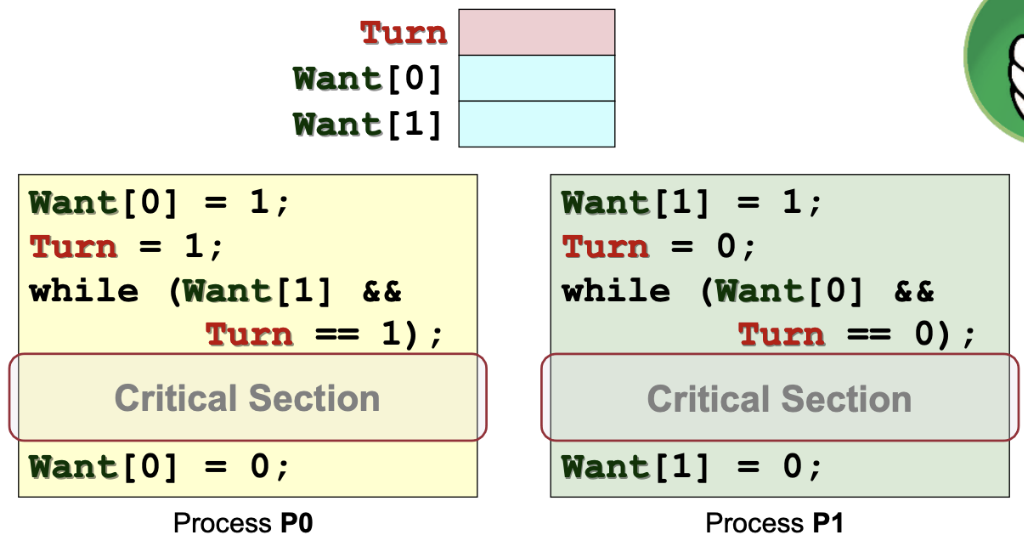
\includegraphics[scale=0.34]{peterson-algorithm}
\begin{itemize}
	\item Assembly implementation
	\begin{itemize}
		\item Atomic instruction to load value and replace value in memory location (\textbf{TestAndSet})
		\item \keyword{Atomicity}{Prevents race condition of process viewing and upon modification, the value changes}
		\item No bounded wait unless fair scheduling algorithm employed
		\item Employs busy waiting still
	\end{itemize}
\end{itemize}
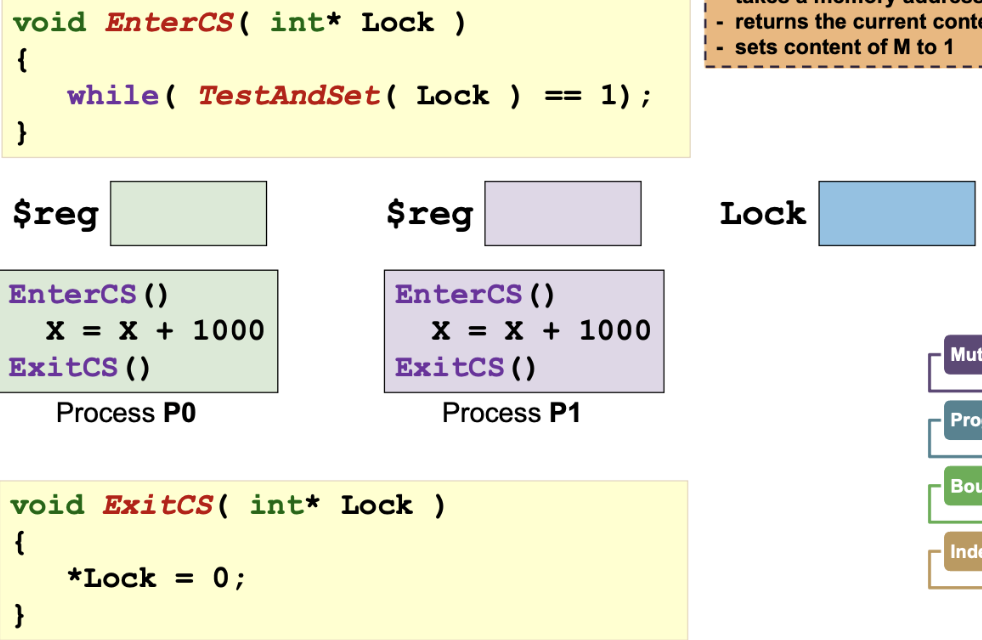
\includegraphics[scale=0.4]{test-and-set}
\begin{itemize}
	\item High level synchronization mechanism (Semaphore)
	\begin{itemize}
		\item Generalised mechanism to block a number of processes (sleeping), $S$, and unblock sleeping processes
		\item \keyword{wait()}{Blocks if $S\leq 0$, decrement S}
		\item \keyword{signal()}{Increment $S$, wake up sleeping processes, operation \textbf{never} blocks}
		\item \keyword{Invariant}{$S_{current} = S_{initial} + N_{signal} - N_{wait}$}
	\end{itemize}
\end{itemize}
\subsubsection{Conditional variables}
\begin{itemize}
	\item Tasks wait for certain events to happen
	\item Event completion/begin is broadcasted
\end{itemize}
\subsubsection{POSIX semaphore}
\begin{description}
	\item[header]{semaphore.h}
	\item[wait]{pthread\_mutex\_unlock}
	\item[signal]{pthread\_mutex\_lock}
\end{description}

%--------------------------------------------------------------------------------------------------------------------
\section{Midterm}
\begin{itemize}
	\item \keyword{Tail-call optimization}{Stack frame can be replaced in iterative recursion since all information is retained in the 'return' function call at every iteration}
\end{itemize}

%--------------------------------------------------------------------------------------------------------------------
\section{07.Threads}
\subsection{Motivation}
\begin{itemize}
	\item Processes are expensive
	\begin{itemize}
		\item Process creation via fork() duplicates memory space and process context
		\item Requires context switching and saving/restoring process information repeatedly
	\end{itemize}
	\item Hard to communicate with each other
	\begin{itemize}
		\item Independent memory space (IPC communication only)
	\end{itemize}
	\item Need easy way to execute some instructions simultaneously (more threads of control to same process)
\end{itemize}
\subsection{Features}
\begin{itemize}
	\item \keyword{Multithreaded process}{Single process with multiple threads}
	\item Threads share the same \textbf{Memory context}(Text, data, heap) and \textbf{OS context}(PID)
	\item Contains unique information
	\begin{itemize}
		\item Identification (thread id)
		\item Registers (GPR and special)
		\item Stack
	\end{itemize}
\end{itemize}

\subsection{Benefits}
\begin{description}
	\item[Economy]{Less resources to manage}
	\item[Resource sharing]
	\item[Responsiveness]
	\item[Scalability]{Can take advantage of multiple CPUs}	
\end{description}

\subsection{Problems}
\begin{itemize}
	\item Syscall concurrency
	\begin{itemize}
		\item Parallel execution of threads may result in parallel syscalls
	\end{itemize}
	\item Process behaviour
	\begin{itemize}
		\item Unable to impact process operations
	\end{itemize}
\end{itemize}

\subsection{Thread implementation}
\begin{itemize}
	\item Threads are \textbf{NOT} new processes
	\item Threads share the same stack, file descriptors and page tables
\end{itemize}

\begin{enumerate}
	\item User thread
	\begin{itemize}
		\item Implemented as a user library -\> More flexible and configurable
		\item Runs on any OS
		\item Kernel unaware of threads in process (scheduling at process level)
		\item If process is blocked, all the threads in the process cannot run 
	\end{itemize}
	\item Kernel thread
	\begin{itemize}
		\item Implemented in the OS through syscalls (slower and more resource intensive)
		\item Scheduling among threads instead of via process
		\item Use threads in kernel operations
		\item Less flexible
		\begin{itemize}
			\item Used by all multithreaded programs so kernel must cater to all
			\item Balance btw many and less features
		\end{itemize}
	\end{itemize}
	\item Hybrid thread
	\begin{itemize}
		\item OS schedules on kernel threads
		\item User threads can be bound to kernel threads
		\item If the user thread is blocked, the kernel thread that it is assigned to is blocked and the OS will execute another kernel thread
		\item Lead to greater flexibility
	\end{itemize}
\end{enumerate}

\subsection{Posix Threads (pthreads)}
\subsubsection{pthread\_create}
\begin{description}
	\item[param]{tid, attributes, \&function, function\_params}
	\item[return]{0 success, != 0 fail}
\end{description}

\subsubsection{pthread\_exit}
\begin{description}
	\item Automatically called after function finishes
	\item[param]{exit\_value}
	\item[behaviour]{return value of function will be the "exit value"}
\end{description}

\subsubsection{pthread\_join}
\begin{description}
	\item[param]{tid, \keyword{\&status}Exit value returned by target pthread}
\end{description}

%--------------------------------------------------------------------------------------------------------------------
\section{08. Classic synchronisation problems}
Use cases of synchronisation (mutexes)

\subsection{Producer Consumer}
\begin{itemize}
	\item Processes share a bounded biffer of size K
	\begin{itemize}
		\item Producers produce items to insert in buffer when not full
		\item Consumers remove items from buffer when non-empty
	\end{itemize}
	\item Busy waiting vs blocking version and message passing
\end{itemize}
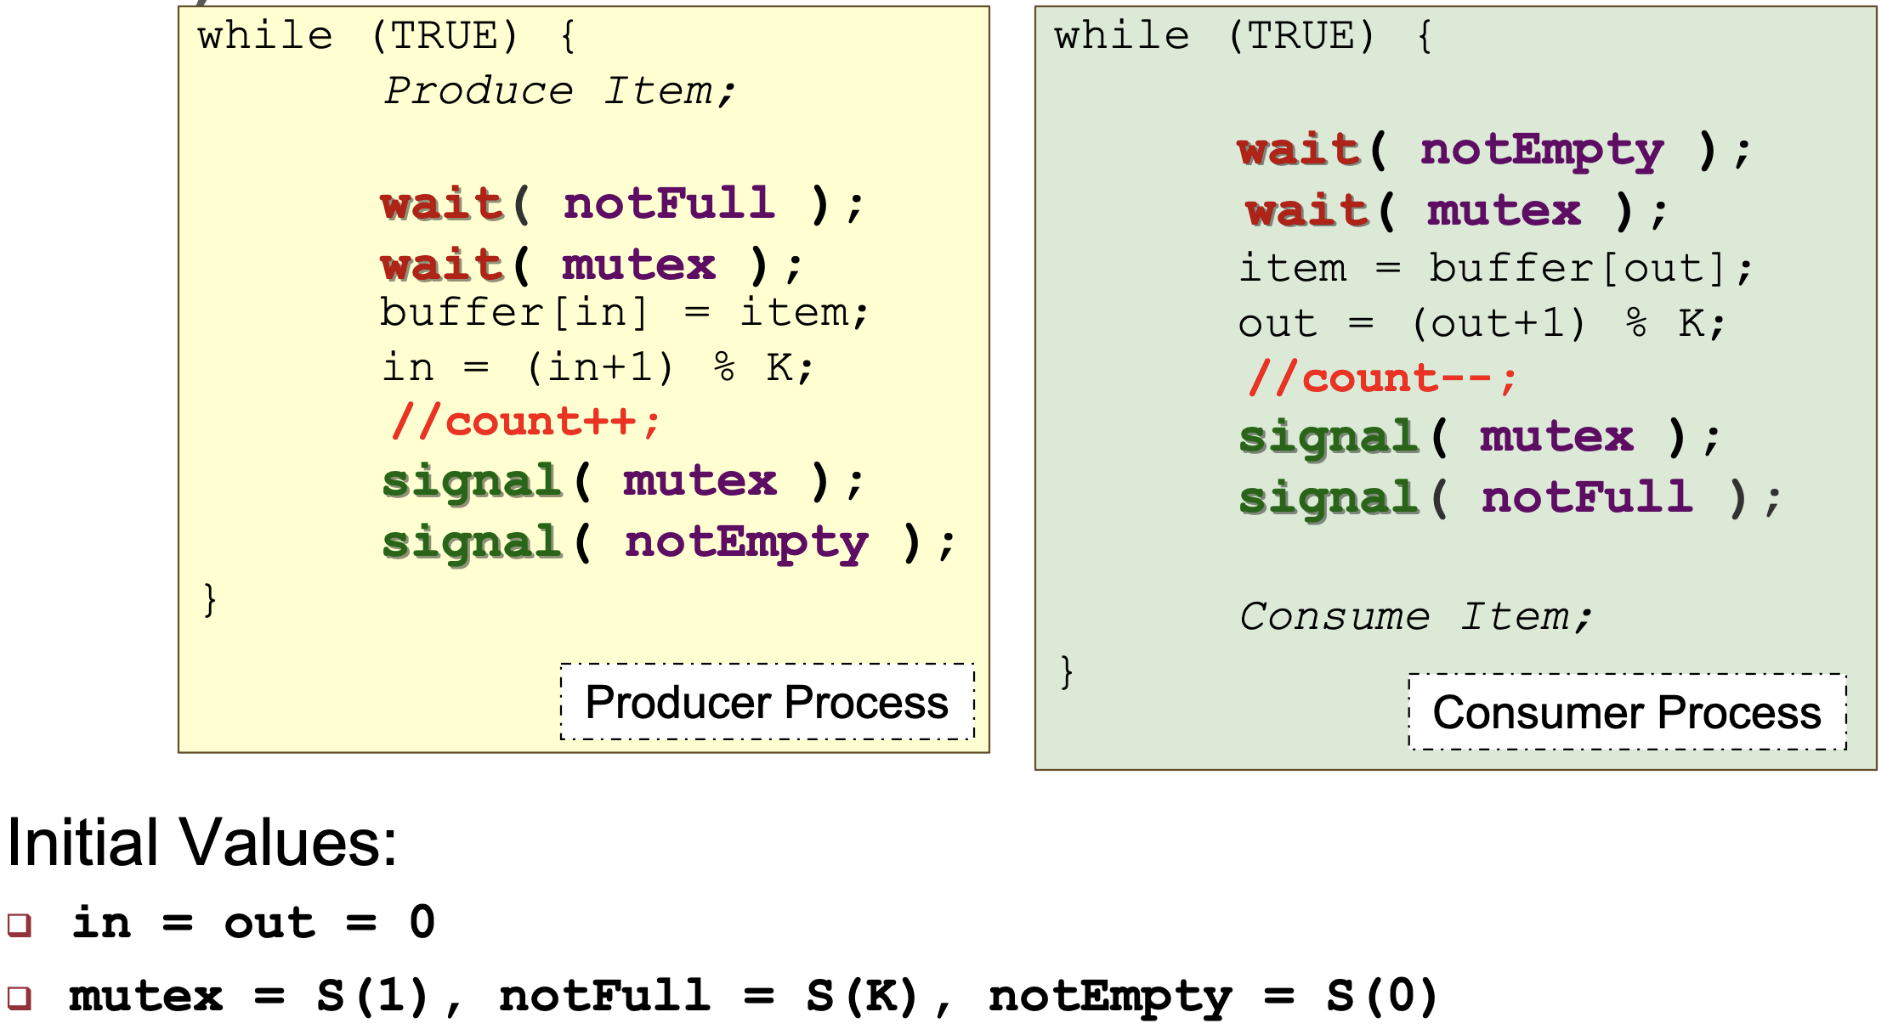
\includegraphics[scale=0.23]{producer-consumer}

\subsection{Reader writer/Barbershop}
\begin{itemize}
	\item Processes share data structure D
	\begin{itemize}
		\item Reader retrieves information from D (multiple concurrent accesses)
		\item Writer modifies information from D exclusively
	\end{itemize}
	\item Starvation of the writer as readers can continue to occupy the resource continuously
\end{itemize}
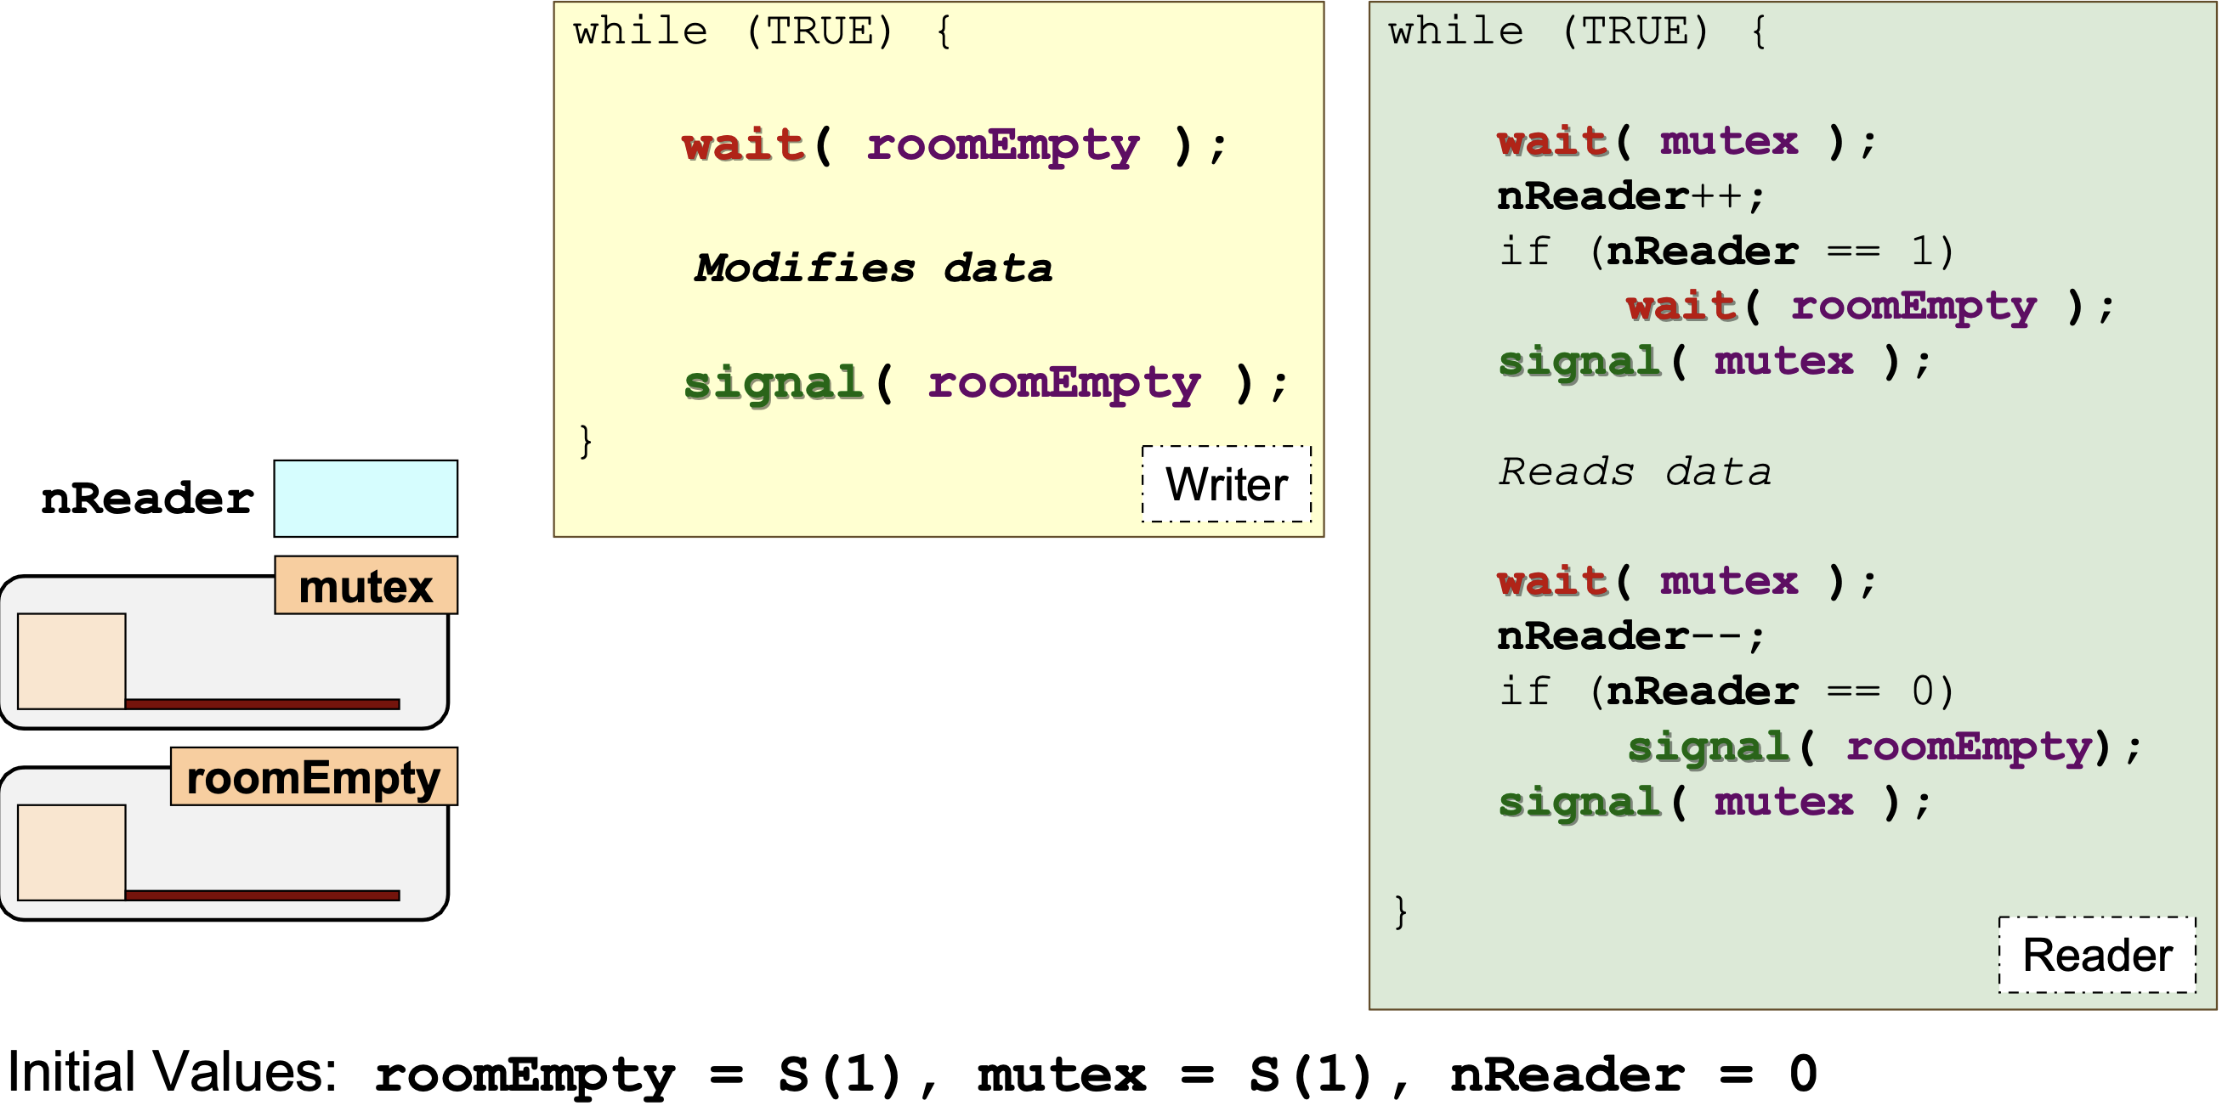
\includegraphics[scale=0.24]{reader-writer}

\subsection{Dining philosophers}
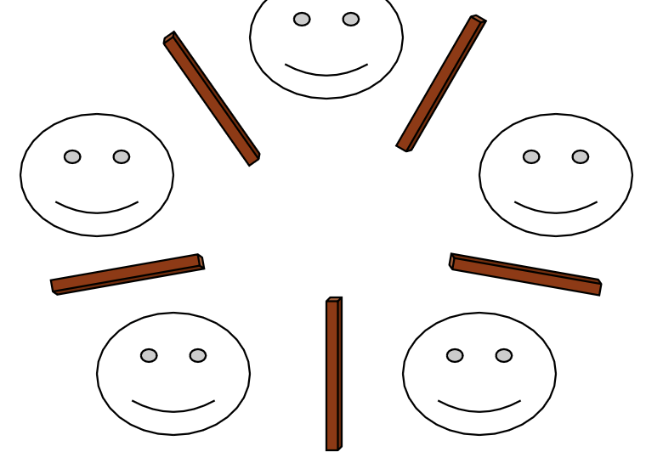
\includegraphics[scale=0.2]{dining-philosophers-spec}
\begin{itemize}
	\item Single chopsticks between philosophers sitting around a table
	\item Philosophers need pair to eat without deadlocks and starvation
	\item Philosophers makes the same decision (takes the same side of chopsticks everytime)
\end{itemize}
\subsubsection{Livelock}
\begin{itemize}
	\item To prevent deadlock, philosophers put down chopstick if cannot get the other side
	\item Livelock because all philosophers take chopstick, put down ....
\end{itemize}

\subsubsection{Limited eater}
\begin{itemize}
	\item One of the philosophers delay their eating temporarily until either side finishes
	\item All philosophers can complete their execution pigeonhole theorum (more chopsticks than philos)
	\item Not fair to the philosopher not eating (How to decide who stops operation?)
\end{itemize}

\subsubsection{Tanenbaum Solution}
\begin{itemize}
	\item Randomly decide which side chopstick the philosophers take first
\end{itemize}
%------------------------------------------------------------------------------------------------------------------------------

\section{09. Memory abstraction}
\subsubsection{Hardware}
\begin{itemize}
	\item uses Random Access Memory
	\begin{itemize}
		\item Access latency approximately constant regardless of location
	\end{itemize}
	\item Can be treated as a 1D array of \keyword{AU}{Addressable unit}
	\item \keyword{Contiguous}{Consecutive memory address with unique index (physical address)}
\end{itemize}
\subsubsection{Content}
\begin{itemize}
	\item Text (for instructions), Data (global variables), Heap (dynamic allocation)
	\item Stack (for function invocation)
	\item Btw heap and stack is region of unallocated memory
\end{itemize}
\subsubsection{Memory usage of process}
Types of data
\begin{enumerate}
	\item \keyword{Transient data}{Valid only for a specific duration (parameters, local var)}
	\item \keyword{Persistent data}{Valid for complete duration of prgm until explicitly deallocated}
\end{enumerate}
\subsubsection{Role of OS}
\begin{enumerate}
	\item Allocate and manage memory space for each process
	\item Protect memory space of distinct processes
	\item Provide memory-related system calls
	\item Manage memory space for internal OS use
\end{enumerate}

\subsection{Memory abstractions}
\subsubsection{Motivation}
\begin{itemize}
	\item Processes assume memory starts at 0 and occupy the same memory location
	\item Difficult to protect memory space
\end{itemize}
\subsubsection{Solutions (?)}
\begin{itemize}
	\item Address reallocation
	\begin{itemize}
		\item Offset all memory references when process is loaded to actual memory address
		\item Problems: Slow runtime because have to run through all the instructions
		\item Difficulty in distinguishing memory references
	\end{itemize}
	\item Base and limit registers
	\begin{itemize}
		\item All memory references compiled as offset from base register
		\item When loading, base register initialised to starting address of process memory space
		\item Limit register as the range of memory space of current process (protect memory space integrity)
		\item Memory access checked against limit
	\end{itemize}
\end{itemize}
\subsubsection{Logical address}
\begin{itemize}
	\item How each process views its memory space
	\item Mapping between physical and logical address needed
	\item Each process has a self contained, independent logical memory space
\end{itemize}
\subsection{Contiguous Memory allocation}
\subsubsection{Assumptions}
\begin{itemize}
	\item Processes occupies contiguous memory region
	\item Physical memory must accommodate 1..* processes with complete memory space
\end{itemize}
\subsubsection{Multitasking/context switching}
\begin{itemize}
	\item Multiple concurrent processes in memory
	\item Free memory via removing terminated processes\slash swapping to secondary storage
\end{itemize}
\subsubsection{Fixed size partitions}
\begin{itemize}
	\item Fixed number of partitions of equal size 
	\item Larger min addressable units of partition 
	\item \keyword{Internal fragmentation} More memory allocated to program than used
	\item Pros: Easy to manage and fast to allocate
	\item Cons: Partition size need to be large enough to contain the largest process
\end{itemize}
\subsection{Variable size partitions}
\keyword{External fragmentation}{Unallocated contiguous memory surrounding partitions insufficient to satisfy memory request of process}
\begin{itemize}
	\item Pros: Flexible, no internal fragmentation
	\item Cons: Need more info in OS and takes longer time to locate appropriate region
\end{itemize}
\subsubsection{Allocation algorithms}
\begin{itemize}
	\item First fit 
	\begin{itemize}
		\item Take the first hole large enough
		\item Fastest runtime (don't have to iterate through all the free partitions)
		\item May be inefficient (high external fragmentation)
	\end{itemize}
	\item Best fit
	\begin{itemize}
		\item Choose the smallest partition that fits the information
		\item Slower runtime but more efficient
	\end{itemize}
	\item Worst fit
	\begin{itemize}
		\item Choose the largest partition 
		\item Try to ensure that there is enough free space in the large partition for other process
	\end{itemize}
\end{itemize}
\subsubsection{Merging and Compaction}
\begin{description}
	\item[Merging] Freed partitions can join surrounding holes
	\item[Compaction] Mv occupied partitions to create bigger consolidated holes
	\begin{itemize}
		\item Time consuming (can be amortised)
	\end{itemize}
\end{description}

\subsection{Multiple free lists}
\begin{itemize}
	\item Dictionary of list of free holes
	\begin{itemize}
		\item Key = size, value = addresses
	\end{itemize}
	\item Find smallest hole that accommodates req size
	\item Partition size increases exponentially 
	\item Faster allocation (vs iterating all holes)
\end{itemize}
\subsubsection{Buddy system}
\begin{itemize}
	\item Free block split into half repeatedly to meet request size
	\item Merge buddy blocks when both free
	\item Efficient partition splitting and dealloc 
	\item Locate good match for holes 
\end{itemize}
\subsubsection{Allocation algorithm}
\begin{itemize}
	\item Free block split half repeatedly to meet req size
	\item Buddy block pair merge when free
\end{itemize}
N = req size, $2^K$ = largest allocable block size\\
A[J] = linked list of free blocks with size $2^J$
\begin{enumerate}
	\item Find smallest s such that $2^s \geq N$
	\item Access A[S] for free block
	\begin{enumerate}
		\item Free block exists
		\begin{itemize}
			\item Remove block from free block list
		\end{itemize}
		\item Find smallest R from S+1 - K such that A[R] has a free block B
		\item Split B and restart from step 2
	\end{enumerate}
\end{enumerate}
\subsubsection{Deallocation algorithm}
\begin{enumerate}
	\item Check if buddy (sizeof=$2^S$) is free in A[S]
	\begin{enumerate}
		\item If buddy is free 
		\begin{itemize}
			\item Remove both blocks from list
			\item Add merged block, B' to A[S+1]
			\item Repeat steps for B'
		\end{itemize}
	\end{enumerate}
\end{enumerate}
2 blocks B and C of size $2^S$ are buddies if
\begin{itemize}
	\item Right S bits (0..S-1) of B and C are identical
	\item S+1th bit of B and C is different
\end{itemize}

\section{10. Disjoint memory schemes}
\begin{itemize}
	\item Processes informations can be split into disjoint physical memory chunks
	\item \keyword{Address space}{Amount of memory allocated for all possible addresses for system}
	\begin{itemize}
		\item "32-bit system" $\rightarrow 2^{32} * $  addressing size = address space 
	\end{itemize}
\end{itemize}
\subsection{Paging scheme}
\begin{itemize}
	\item \keyword{Physical frames}{Phy mem split into regions of fixed size}
	\item Frames sizes are decided by hardware (CPU)
	\begin{itemize}
		\item Reduce number of access to memory
		\item Dedicated component to support paging by speeding address translation
	\end{itemize}
	\item \keyword{Logical page}{Logical mem split into regions of same size}
	\item Pages of process loaded into any available mem frame at execution time
	\item Logical mem remains contiguous
\end{itemize}
\subsubsection{Page table - Lookup mechanism}
\begin{itemize}
	\item Map logical pages to physical frames
	\item Frame sizes should be power of 2 
	\item $size_{page\_table} * s_{page} = s_{mem\_address} * s_{entry} * s_{addressing}$
\end{itemize}
\subsubsection{Translation}
%\begin{itemize}
%	\item Logical address = Page num + offset
%	\item Page num = $m-n$ most significant bits
%	\item $2^n$ = frame size, m = logical add size
%	\item page num $\rightarrow$ frame num via table
%	\item Physical address = Frame num + offset
%\end{itemize}
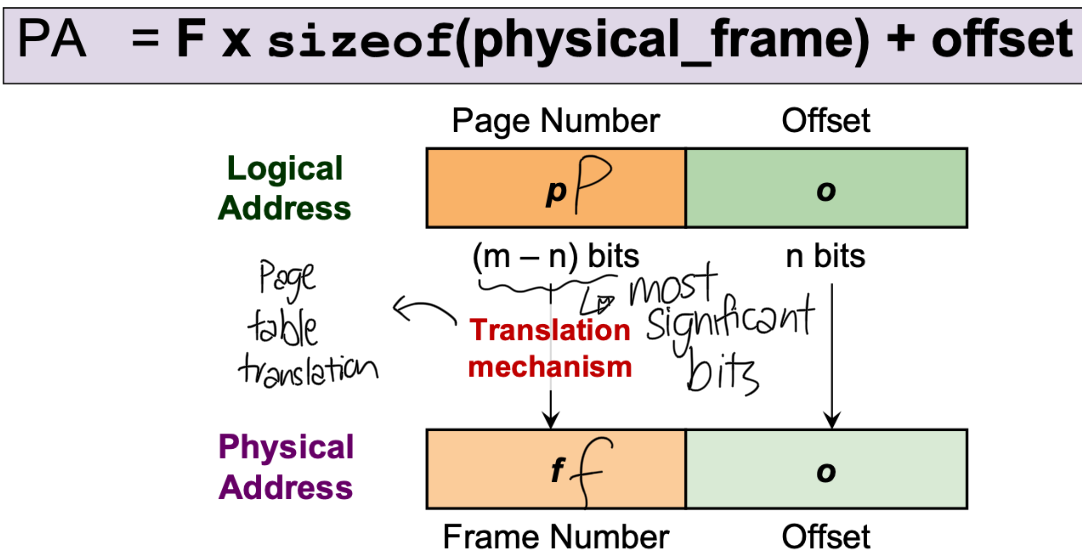
\includegraphics[scale=0.3]{paging-translation}
\subsubsection{Benefits}
\begin{itemize}
	\item No external fragmentation 
	\begin{itemize}
		\item Every single free frame can be used
	\end{itemize}
	\item Insignificant internal fragmentation
	\item Separation of logical and physical address
	\begin{itemize}
		\item Greater flexibility
		\item Simple translation
	\end{itemize}
\end{itemize}
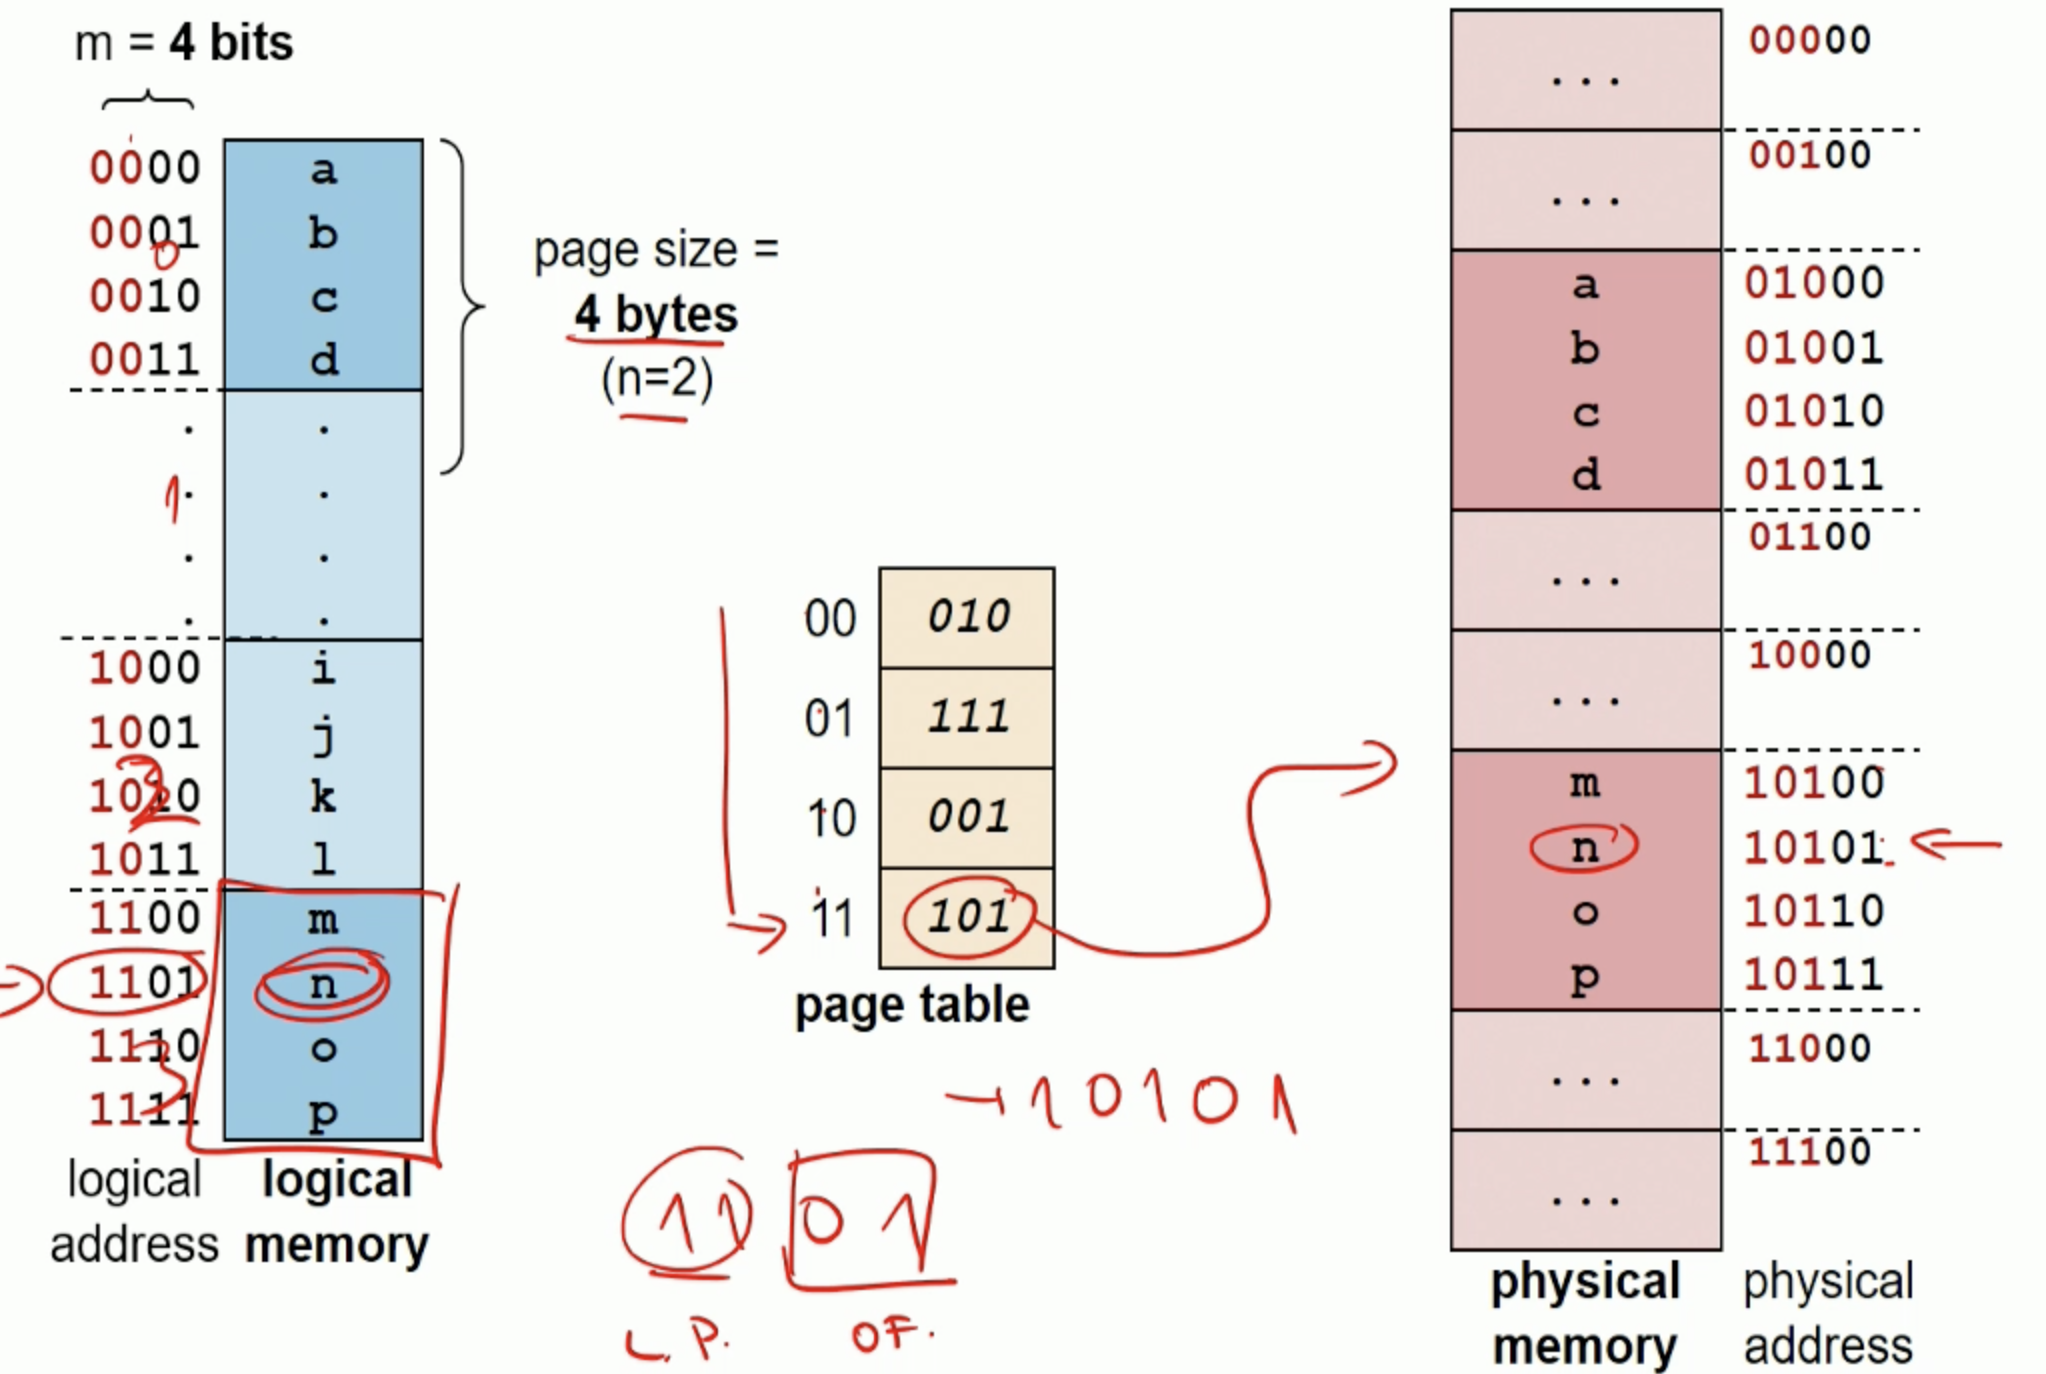
\includegraphics[scale=0.2]{paging-example}
\subsubsection{Implementation}
\begin{enumerate}
	\item Pure software solution
	\item Page table info in Process Control Block (PCB)
	\begin{itemize}
		\item 2 mem access per reference
		\begin{enumerate}
			\item Read the indexed page table entry to get the frame number
			\item Access the actual memory item
		\end{enumerate}
	\item Memory context of process includes page table\slash pointers to it
	\end{itemize}
	\item Hardware support
	\begin{itemize}
		\item Contain \keyword{Translation Look-aside Buffer}{Specialized on-chip component to cache page table entries}
		\item Use page numbers to search TLB associatively
		\item Possible to have multiple TLB per core
		\begin{description}
			\item[TLB-hit]{Frame number retrieved to generate physical address}
			\item[TLB-miss]{Memory access to page table $\rightarrow$ frame number used to generate physical address and update TLB}
		\end{description}
		\item Very small and fast (reducing Average Memory Access Time)
		\begin{itemize}
			\item AMAT = $P(TLB~hit)*latency(TLB~hit)+P(TLB~miss)*latency(TLB~miss)$
			\item Latency of filling in TLB hidden by hardware
		\end{itemize}
		\item Part of hardware context, so entries will be flushed when context switch occurs
		\begin{itemize}
			\item Save pointer to prev process' page table in PCB 
			\item Ensure process does not get incorrect translation
		\end{itemize}
	\end{itemize}
\end{enumerate}

\subsubsection{Protection}
\begin{itemize}
	\item Access-right bits
	\begin{itemize}
		\item Enforce protection like read, write execute permissions
		\item Memory access checked against access-right bits in hardware
	\end{itemize}
	\item Valid Bit
	\begin{itemize}
		\item Exclude pages that are out-of-range for particular process from mapping
		\item Check against bits in hardware whether the page can be accessed by process
	\end{itemize}
\end{itemize}
\subsubsection{Page sharing}
\begin{itemize}
	\item Several processes' logical pages mapped to same physical frame
	\begin{itemize}
		\item Used in shared code pages - code used by many processes
		\item Implementing copy on write - pages shared until child changes its value
	\end{itemize}
\end{itemize}


\subsection{Segmentation scheme}
\subsubsection{Motivation}
\begin{itemize}
	\item Process contains different types of memory regions (data, text, heap, stack)
	\begin{itemize}
		\item Order of memory regions does not matter
	\end{itemize}
	\item Regions are variable sized and grow/shrink at execution time 
	\begin{itemize}
		\item Gaps btw regions shld be provisioned early
		\item Difficult to check the permissions of memory access (which range it is)
	\end{itemize}
\end{itemize}
\subsubsection{Implementation}
\begin{itemize}
	\item Process broken into named segments of variable sizes
	\item Manage memory at level of memory segments
	\item Segments itself are mapped to contiguous physical partitions
	\begin{itemize}
		\item base address and limit (range of segment)
	\end{itemize}
	\item Logical address $<$SegID\slash name, Offset$>$
	\begin{itemize}
		\item SegID used to find $<$Base add, Limit$>$ in segment table
	\end{itemize}
\end{itemize}
\subsubsection{Evaluation (Pros and Cons)}
\begin{itemize}
	\item[+] Independent contiguous memory space matches programmers view of memory
	\item[+] More efficient bookkeeping
	\item[+] Segments can grow/shrink and be protected/shared independently
	\item[-] Cause external fragmentation due to variable sized contiguous memory regions
\end{itemize}
\subsection{Segmentation with paging}
\begin{itemize}
	\item Each segment contains fixed sized pages with its own page table
	\item Segment grows by allocating new page and adding to its page table 
\end{itemize}
\section{11. Virtual Memory Management}
\subsection{Motivation}
\begin{itemize}
	\item Logical memory space may be $>>$ than phy mem
	\item Not portable to different phy memory sizes
\end{itemize}
\subsubsection{Advantages}
\begin{itemize}
	\item Security: Cannot be corrupted by other processes
	\item Efficient for caching virtual mem pages (locality)
	\item Simplify memory management, programming and protection
	\item Memory sharing
\end{itemize}
\subsection{Extension of paging scheme}
\begin{itemize}
	\item Split logical address space into fixed size pages
	\begin{itemize}
		\item May reside in phy mem or secondary storage
	\end{itemize}
	\item 2 new page types to denote phy location of information
	\begin{description}
		\item[Memory resident]{Pages in phy memory stored in kernel space}
		\item[Non-memory resident]{Pages in secondary mem}
		\item \keyword{Resident bits}{Used to denote whether resident in mem}
	\end{description}
	\item \keyword{Page fault}{CPU access non-memory resident page}
	\begin{itemize}
		\item CPU can only access mem resident pages - blocks process
		\item OS needs to bring pages from secondary storage to phy mem 
	\end{itemize}
\end{itemize}
\subsubsection{Execution}
\begin{enumerate}
	\item{Check page table if page is mem resident}
	\begin{itemize}
		\item[+]{Access phy mem loc directly}
		\item[-]{Throw page fault \textbf{exception}}
	\end{itemize}
	\item Locate page in secondary memory
	\item Load page into phy memory
	\item Update page table
	\item Re-execute step 1 with mem-resident page
\end{enumerate}
\subsubsection{Page Fault}
\begin{itemize}
	\item Page transfer is I/O operation done by DMA controller
	\begin{itemize}
		\item Direct Access Media - abstract I/O from CPU
	\end{itemize}
	\item Faulted process is in \textbf{blocked} state
	\item May send SIGSEGV if accessing mem region without access rights
	\begin{itemize}
		\item Sig thrown when offset $>$ page size
	\end{itemize}
	\item \keyword{Thrashing}{System slow down due to multiple page faults}
\end{itemize}
\subsubsection{Locality}
\begin{description}
	\item[Temporal]{Mem address likely used multiple times}
	\item[Spatial]{Adjacent mem address likely accessed soon}
\end{description}
\subsection{Paging scheme}
\subsubsection{Objectives}
\begin{itemize}
	\item Reduce startup cost when allocating pages during initialization
	\item Reduce footprint of processes in phy mem
\end{itemize}
\subsubsection{Demand Paging}
\begin{itemize}
	\item Only allocate mem resident pages when page fault
	\item Processes start with no mem resident pages
	\item[+]{Fast startup time and small mem footprint}
	\item[-]{Sluggish proc initially due to multiple page faults}
	\item[-]{Thrash other processes during page fault}
\end{itemize}
\subsection{Page table structure}
\subsubsection{Consideration}
\begin{itemize}
	\item Large logical and phy mem space $\rightarrow$ Large page size
	\item Every proc needs a page table (pointer in register)
	\item Minimize page table size
	\begin{itemize}
		\item High overhead 
		\item Page table may occupy several frames (Difficult to keep track locations)
	\end{itemize}
\end{itemize}
\subsubsection{2-level paging}
\begin{itemize}
	\item Split page table into regions with page table num
	\item Regions allocated when mem usage grows
	\item Page directory in PCB keeps track of smaller page tables
	\item Memory context of process only stores the page directory
\end{itemize}
\textbf{Problems}
\begin{itemize}
	\item 2 serialized memory access to get frame number
	\begin{itemize}
		\item MMU cache frequent page directory entries
		\item Speed up page-table walk upon TLB miss
		\item Usual: log$\rightarrow$page directory$\rightarrow$page table$\rightarrow$phy frame
		\item MMU: log page$\rightarrow$page-table$\rightarrow$phy frame
		\item TLB: log page$\rightarrow$phy frame
	\end{itemize}
\end{itemize}
\subsubsection{Inverted Page Table}
\begin{itemize}
	\item Map physical frames to $<$pid, page number$>$
	\item Upper bound on table size (limited to num phy frames)
	\item One table for all processes but slow translation
	\begin{itemize}
		\item Need search whole table to find the phy frame that has the specific page
	\end{itemize}
	\item Does not support memory page sharing
\end{itemize}

\subsection{Page Replacement Algorithms}
\begin{itemize}
	\item Deciding the phy memory frame to \textit{evict} during page fault
	\item $T_{mem~access}=(1-p)T_{mem}+p*T_{page~fault}$
	\begin{itemize}
		\item p = probability page fault, $T_mem$ = access time for mem resident page
	\end{itemize}
\end{itemize}
\subsubsection{Optimal Page Replacement}
\begin{itemize}
	\item Replace page that will not be needed again for longest period of time
	\item[-] Impossible to know future memory references
\end{itemize}
\subsubsection{FIFO Page Replacement}
\begin{itemize}
	\item Evict oldest loaded memory page
	\item Maintain queue of resident page numbers and update queue during page faults
	\item \keyword{Belady's Anomaly}{More physical frames the higher likelihood of page faults}
	\begin{itemize}
		\item FIFO does not exploit temporal locality (commonly used frames evicted)
	\end{itemize}
\end{itemize}
\subsubsection{Least Recently Used (LRU)}
\begin{itemize}
	\item Replace page that has not been used in the longest time
	\item OS keeps track of last access time
	\item Logical Time counter incremented for every mem reference
	\begin{itemize}
		\item Page table entry has a time-of-use field which increases when referenced
		\item Replace pages that have the smallest TOU
		\item O(n) operation and overflow possible (TOU strictly increasing)
	\end{itemize}
	\item Maintain stack of page numbers
	\begin{itemize}
		\item Page removed from stack and pushed to top when referenced
		\item Replace page at bottom of stack during replacement
		\item Hard to implement in hardware (entries removed randomly)
	\end{itemize}
	\item Second-Change Page Replacement\slash CLOCK
	\begin{itemize}
		\item Modified circular FIFO to give second chance to pages accessed
		\item Every PTE maintains \keyword{Reference bit}{1= accessed since last reset}
	\end{itemize}
	\begin{enumerate}
		\item Oldest FIFO page is selected
		\item If ref bit == 0: page replaced, else..
		\item Page is skipped
		\begin{itemize}
			\item Ref bit cleared to 0 
			\item \textbf{NOTE!!} Page does not refresh its position in queue
			\item Next FIFO page selected\slash given chance
		\end{itemize}
	\end{enumerate}
\end{itemize}
\subsubsection{Page Replacement}
\begin{description}
	\item[Victim page]{Page that will be replaced}
	\item[Global]{Victim page chosen among all physical frames}
	\begin{itemize}
		\item \keyword{Self adjustment}{Processes that need more frames can get more}
		\item Badly behaved processes affect others
		\item Non-deterministic number of frames allocated to processes during each run
	\end{itemize}
	\item[Local]{Victim page chosen from pages of process that caused page fault}
	\begin{itemize}
		\item More stable - number of frames allocated to each process remain constant 
		\item Frame allocation matters - progress of process may be hindered
	\end{itemize}
\end{description}
\subsection{Frame Allocation}
\begin{itemize}
	\item How to distribute N physical memory frames among M processes	
\end{itemize}
\subsubsection{Approach}
\begin{description}
	\item[Equal]{Every process gets equal num frames $N/M$}
	\item[Proportional]{Each process, P gets $\dfrac{size_p}{size_{total}}*N$}
\end{description}
\subsubsection{Problems}
\begin{itemize}
	\item Difficulty in finding right number of frames to prevent thrashing
	\item \keyword{Cascading thrashing}{Process steals page alloc from other proc}
	\item I/O bandwidth costly and may degrade performance 
\end{itemize}
\subsubsection{Working Set Model}
\begin{itemize}
	\item \keyword{Working set}{Set of pages referenced by process during a period of time}
	\item Working set may changes continuously but is relatively constant
	\item Model aims to find a good window to reduce possibility of page faults 
	\item $W(t,\triangle)$ = pages in interval at time t, $\triangle$ = window size
	\item \keyword{Transient region}{Working set continuously changing in size}
	\item \keyword{Stable region}{Working set stays the same for a long time}
\end{itemize}


\section{12. File System}
\subsection{Introduction}
\subsubsection{Motivation}
\begin{itemize}
	\item Volatile physical memory so external storage needed for longer term storage
	\item Storage media is not portable 
	\begin{itemize}
		\item Dependent on hardware specification and organisation
	\end{itemize}
\end{itemize}

\subsubsection{Services}
\begin{itemize}
	\item Provides abstraction on top of physical media
	\item High level resource management scheme
	\item Protection between processes and users
	\item Sharing between processes and users
\end{itemize}

\subsubsection{Objectives}
\begin{description}
	\item[Self-contained]{Information stored on media is enough to describe organisation (plug and play)}
	\begin{itemize}
		\item System knows how to read and write information on the storage system automatically
	\end{itemize}
	\item[Persistent]{Retain and be retrieved beyond the lifetime of OS and processes}
	\item[Efficient]{Good management of free and used space while having low overhead for bookkeeping information}
\end{description}
\subsubsection{Memory vs File System management}
\begin{tabular}{|p{45pt}|p{100pt}|p{95pt}|}
\hline
&Memory Management & File System Management\\
\hline
Underlying Storage&Ram&Disk\\
\hline
Access speed&Constant&Variable Disk I/O time\\
\hline
Unit of addressing&Phy mem address&Disk sector\\
\hline
Usage&Address space for process, Implict when process runs&Non-volatile data,Explicit access\\
\hline
Organization&Paging\slash Segmentation determined by OS and hardware&Different FS:ext(Linux), FAT(windows), HFS(mac)\\
\hline
\end{tabular}

\subsection{File}
\subsubsection{Objective}
\begin{itemize}
	\item Abstraction for logical unit of information by processes
	\item Contains information structured in specific styles
\end{itemize}
\subsubsection{Metadata}
\begin{itemize}
	\item Additional information associated with the file
\end{itemize}
\begin{description}
	\item[Name]{Human readable reference to the file}
	\begin{itemize}
		\item Consistent naming rule
		\item Case sensitivity, length of name, allowed symbols
		\item File extension (sometimes used to indicate file type)
	\end{itemize}
	\item[Identifier]{Unique id for the file used internally by FS}
	\item[Type]{eg. directory, text, object, executable}
	\begin{itemize}
		\item May have a predefined internal structure that must be processed by specific program (jar, pdf)
		\item Distinguishing Type is OS dependent (some use file extensions and some \keyword{magic numbers}{Embedded info in the file stored at the beginning})
	\end{itemize}
	\item[Size]
	\item[Protection]{Classified under reading writing and execution rights for owner, group, and everyone}
	\begin{itemize}
		\item Types of access: Read, write, execute, append, delete, list (read metadata of file)
		
		\item \keyword{access control list}{List of user identity and allowed access types (very customisable but too much overhead)}
		\item \keyword{permission bits}{Classify users into 3 classes (owner, group and all) and define permissions RWX for the classes}
		\begin{itemize}
			\item Command: getfacl (get file acl)
		\end{itemize}
	\end{itemize}
\end{description}

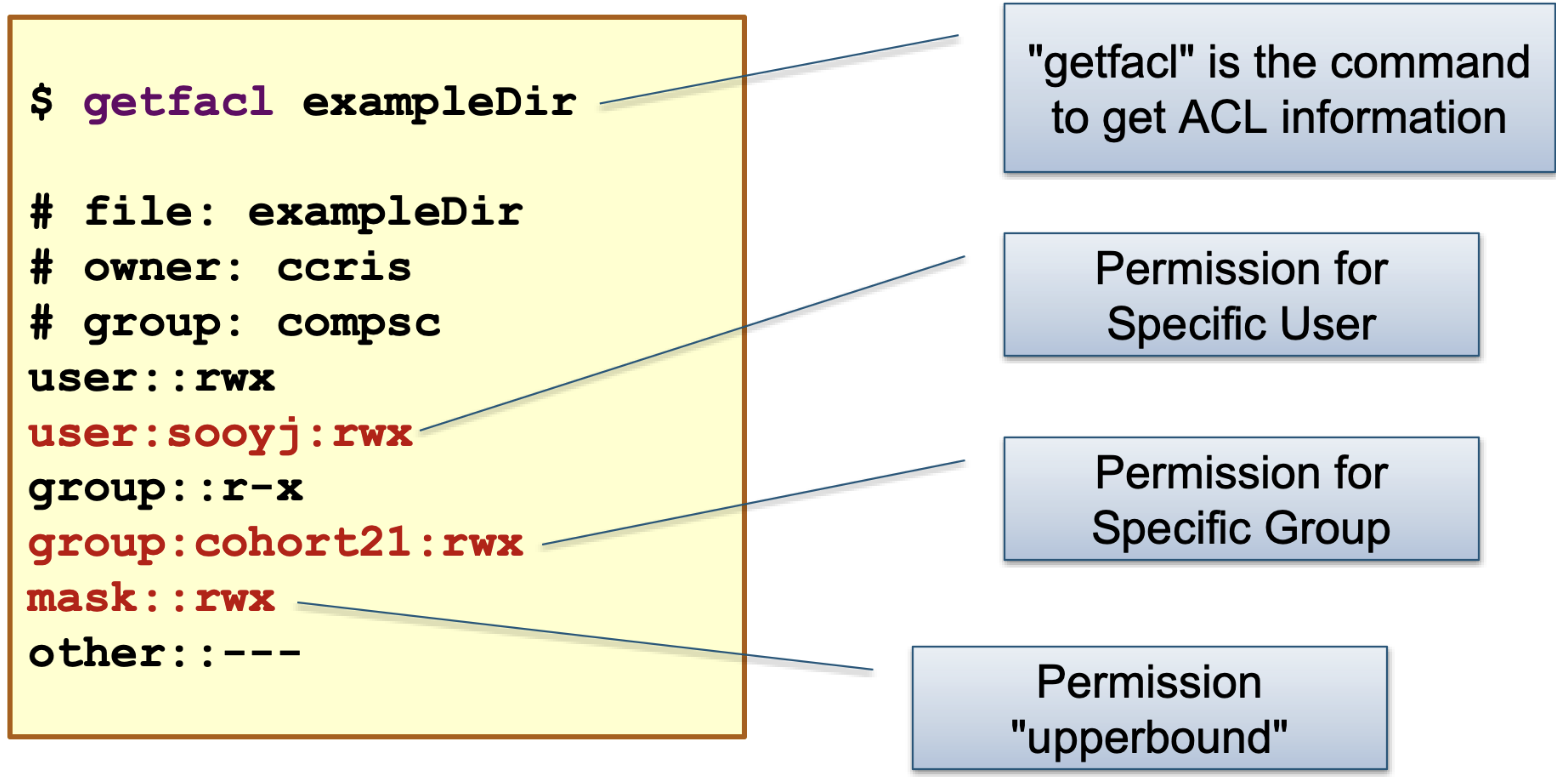
\includegraphics[scale=0.22]{getfacl}
\begin{description}
	\item[Time, date and owner info]
	\item[Table of content]{Info for the FS on how to access the file}
\end{description}
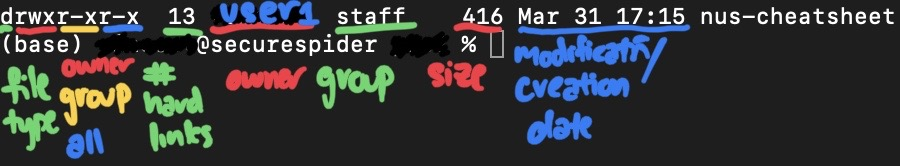
\includegraphics[scale=0.27]{ls-la} %removable

\subsubsection{Types of file structures}
\begin{itemize}
	\item Array of bytes (every byte is addressed by a specific offset from the file start)
	\item Fixed length record
	\begin{itemize}
		\item Array of records that grows and shrinks dynamically
		\item Can jump to Nth offset of M record
		\item Prone to internal fragmentation due to fixed size records
	\end{itemize}
	\item Variable length records
	\begin{itemize}
		\item Flexible size and saves space but harder to locate record
		\item Incurs some overhead and external fragmentation
	\end{itemize}
\end{itemize}


\subsubsection{Access methods}
\begin{description}
	\item[Sequential]{Data read in order and cannot be skipped}
	\item[Random access]{Read bytes in any order}
	\begin{itemize}
		\item Can be read to specific (absolute) offset 
		\item Seek to relative offset from current pointer location (used by unix and windows)
	\end{itemize}
	\item[Direct access]{Random access to any record directly (Fixed length records}
\end{description}

\subsubsection{Operations}
\begin{description}
	\item[Create, read, write]
	\item[Open]{Performed before any operation to prepare necessary info for file operations}
	\item[Repositioning\slash Seek]{Move current position to new location}
	\item[Truncate]{Removes data from specified position to end of file}
\end{description}
\begin{itemize}
	\item Done as system calls to OS for protection, concurrent efficient access
	\item Commands: `open` `read` `write` `lseek` `close`
\end{itemize}
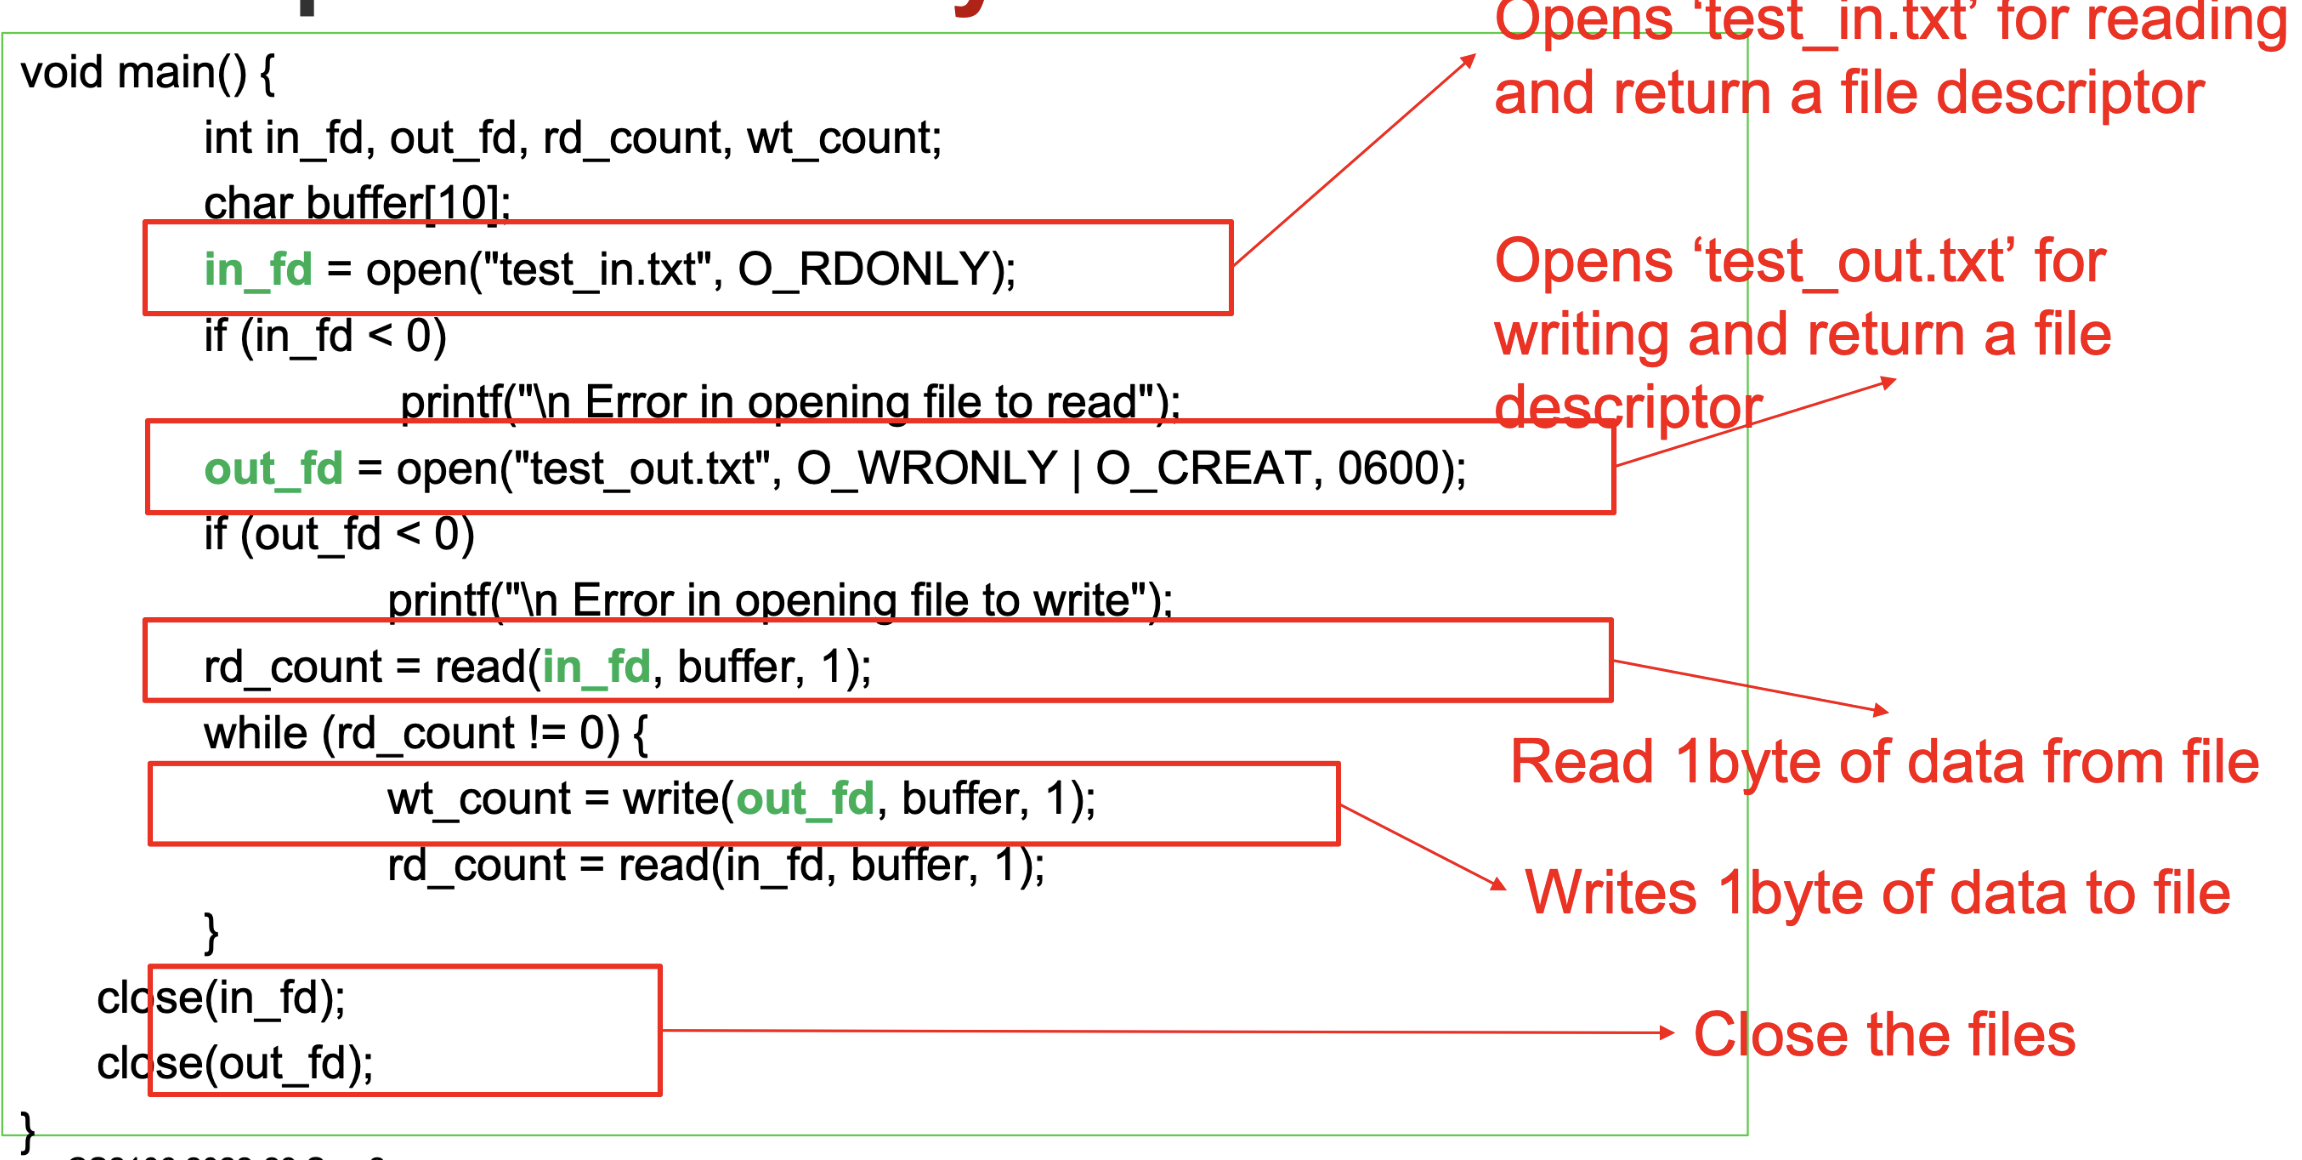
\includegraphics[scale=0.22]{c-file-operations}

\subsection{Implementation in OS}
\subsubsection{Information}
\begin{description}
	\item[File pointer]{Keeps track of current position within a file}
	\item[File descriptor]{Unique identifier of file (int) Used internally in software rather than the name}
	\item[Disk location]{Actual file location on disk}
	\item[Open count/reference count]{How many process opened this file}
\end{description}
\textbf{Criteria}
\begin{itemize}
	\item Multiple processes can open same file
	\item Multiple files can be opened concurrently
\end{itemize}

\subsubsection{Approach}
Using 3 tables to store information
\begin{enumerate}
	\item File is opened twice (can be same process)
	\begin{itemize}
		\item IO occurs at independent offsets
		\item 2 per-proc and 2 sys-wide w diff FD
	\end{itemize}
	\item Multiple proc using same open file table entry
	\begin{itemize}
		\item Forks duplicate file descriptor (share offset)
		\item Only one offset (IO change offset for both proc)
		\item 2 per proc, same FD and sys-wide table
	\end{itemize}
\end{enumerate}
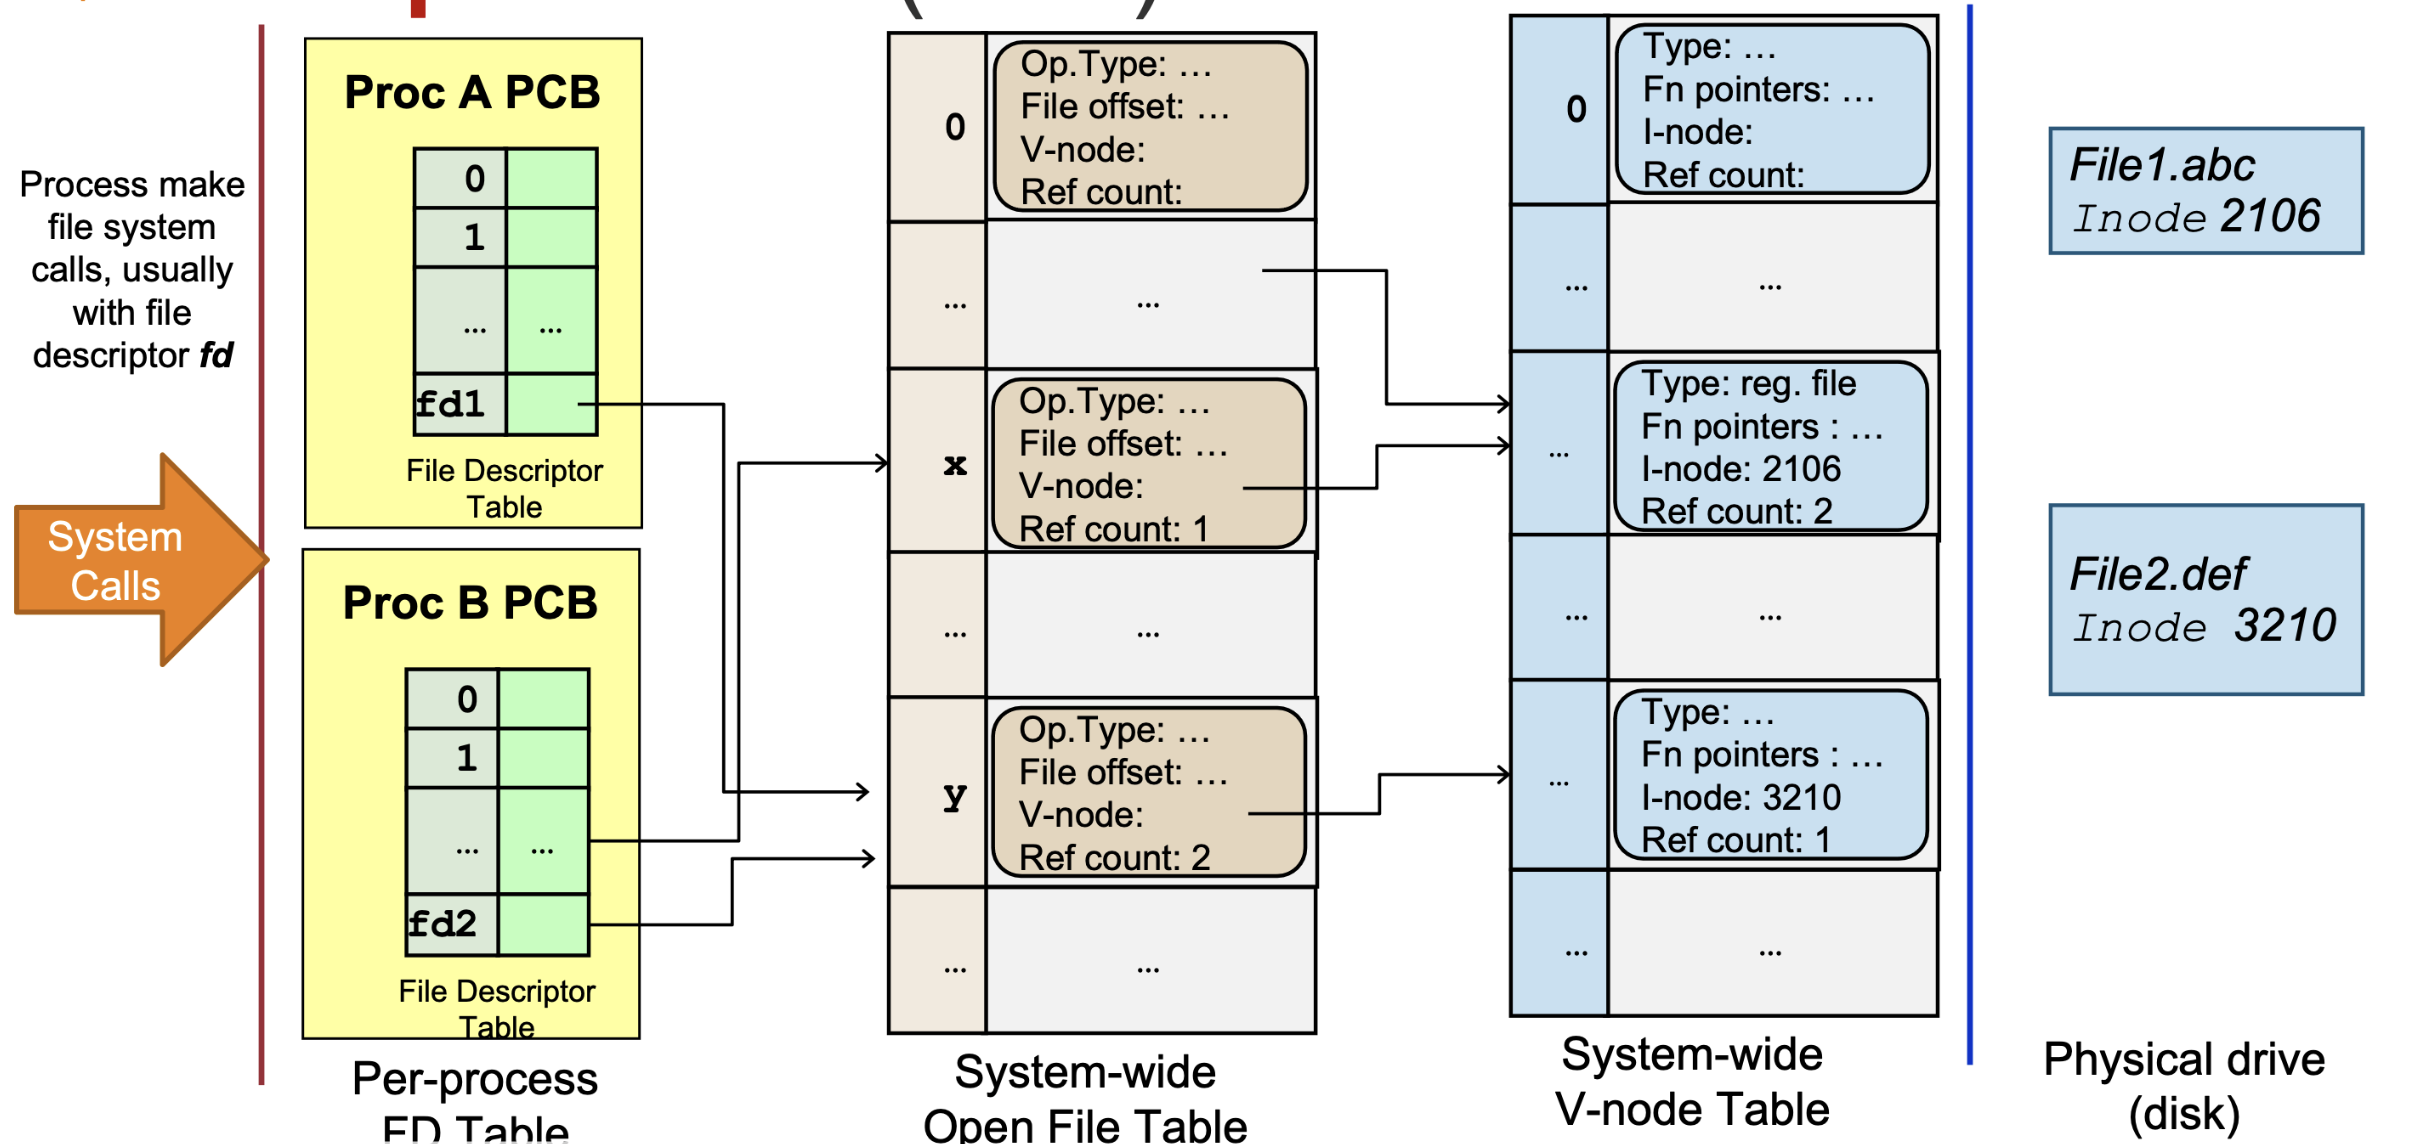
\includegraphics[scale=0.23]{file-system-table-example}
\subsection{Mmap}
\begin{itemize}
	\item Map a shared memory region or share files to multiple process
	\item Both process can access shared data on RAM without system calls
\end{itemize}
\subsection{Directory}
\subsubsection{Motivation}
\begin{itemize}
	\item Provides logical grouping of file
	\item Keep track of files (system usage of directory)
\end{itemize}

\subsubsection{Structure}
\begin{itemize}
	\item Single level
	\begin{itemize}
		\item All files in one directory (CD etc)
	\end{itemize}
	\item Tree structure
	\begin{itemize}
		\item Recursively embedded in other directory
		\item Addressed by absolute or relative pathnames from curr working dir 
	\end{itemize}
	\item DAG
	\begin{itemize}
		\item File can be shared using hard links (dir not allowed)
		\item Shared file appearing in multiple directory referring to the same content using pointers
		\item Low overhead (only pointers added) but deletion problems (synchronisation)
		\item Hard link "ln" command (dir not allowed)
	\end{itemize}
	\item General graph
	\begin{itemize}
		\item Undesirable structure - hard to traverse (cycles)
		\item Hard to determine when to remove file
		\item Implementation via symbolic links (dir allowed)
		\item Sym link is a special link file that contains the path name of file F -\> find out where F is and access it
		\item Deletion is easy as only the special link file is deleted OR dangling link created (link without file)
		\item Larger overhead as special link file is taking up actual disk space
		\item Command: ln -s (cat and vim acts on the target file)
	\end{itemize}
\end{itemize}

\subsection{File system implementation}
\begin{itemize}
	\item Stored as 1-D logical blocks mapped into disk sector organised with unique ID
	\item Storage contains Master Boot Record (MBR) and $\geq1$ partitions
\end{itemize}
\subsubsection{MBR}
\begin{enumerate}
	\item \keyword{Simple boot code}{Defines the partition to be initialised first}
	\item \keyword{Partition table}{Starting and ending address of each partition}
\end{enumerate}

\subsubsection{Partitions}
Partitions can contain independent file systems and OS
\begin{description}
	\item[OS boot block]{All information needed to boot OS from the partition into memory}
	\item[Partition details]{Metadata of partition, loc and num blocks used\slash free etc}
	\item[Directory structure, files info and file data]
\end{description}

\section{13. File System Implementation}
\subsubsection{Objectives}
\begin{itemize}
	\item Keep track of logical blocks
	\item Allow efficient access and utilise disk space effectively
\end{itemize}
\subsection{Allocation Policies}
\subsubsection{Contiguous}
\begin{itemize}
	\item Allocate consecutive disk blocks to a file
	\item Simple to keep track and fast (only need to keep track of the first block)
	\item External fragmentation because file size must be specified in advance
\end{itemize}
\subsubsection{Linked list of disk blocks}
\begin{itemize}
	\item Stores pointer to the next disk block number and actual file data
	\item Need to keep track of the first and last disk block number
	\item Solves fragmentation but random access of file is very slow
	\item Overhead with storing next block number
	\item Less reliable (if one of the pointer breaks, all break)
\end{itemize}
\subsubsection{File Allocation Table (FAT)}
\begin{itemize}
	\item All "next block" pointers stored in a single table rather than at each data block
	\item Table always in memory so simple and efficient (faster random access)
	\item Keeps track of all disk blocks in partition which may waste a lot of memory (valuable)
\end{itemize}

\subsubsection{Indexed allocation}
\begin{itemize}
	\item Each block has index block
	\item Index block records pointers (and index) of blocks in file 
	\item Lower memory overhead (only index block of opened file needs to be in memory)
	\item Faster direct access
	\item Have maximum file size (limited by number of indexes in index block)
	\item Index block overhead (waste one block for indexing)
\end{itemize}
\begin{normalsize}
\textbf{Modified Index Allocation}
\end{normalsize}
\begin{description}
	\item[Linked scheme]{Linked list of index nodes (normal)}
	\item[Multilevel index]{Hierachial linked list (entries point to another linked list of nodes..)}
	\item[Combined]{Direct and multi-level index schemes}
	\begin{itemize}
		\item Fast access for small files and accomodates larger files
	\end{itemize}
\end{description}

\subsection{Partition Details}
\subsubsection{Free Space Management}
\begin{itemize}
	\item Maintain free space info (where and how much, remove/add when file created/deleted)
	\item \keyword{Bitmap}{Disk block represented by bits (1 if free)}
	\begin{itemize}
		\item Mem overhead - complete data structure has to be kept in memory
	\end{itemize}
	\item \keyword{Linked List}{Each disk block contains some free disk blocks/pointer to next free space}
	\begin{itemize}
		\item Easy to locate free block and only one pointer needed in memory
		\item BUT high overhead
	\end{itemize}
\end{itemize}

\subsection{Directory Info}
\subsubsection{Objectives}
\begin{itemize}
	\item Keep track of files in directory and metadata
	\item Map file name to file information
	\begin{itemize}
		\item Locate the file information using pathname and file name to open for use
		\item Parse the full path name by recursively searching directories along path
	\end{itemize}
\end{itemize}
\subsubsection{Linear List}
\begin{itemize}
	\item Each entry represents a file incl name + other metadata + file info/pointer to file info
	\item Locating file requires a linear search
	\begin{itemize}
		\item Inefficient for large directories requiring deep tree traversals
		\item Latest searches can be cached to improve latency
	\end{itemize}
\end{itemize}
\subsubsection{Hash tables}
\begin{itemize}
	\item Every directory contains hash table indexed by filename (with chained collision resolution)
	\item Fast lookup but may be limited in size and dependent on hash functions (to reduce collisions)
\end{itemize}
\subsection{FAT}
\begin{itemize}
	\item Used by Microsoft with 2 main structures (directory and data)
	\item File data allocated to blocks with allocation info kept as linked list
	\item Data block pointers in File Allocation Table with block info (free\slash next occupied block\slash EOF\slash unusable)
	\item OS cache table in Ram to facilitate linked list traversal
	\item Each partition contains the boot, FAT, root directory and multiple data blocks
\end{itemize}
\subsubsection{Directory Structure}
\begin{itemize}
	\item Special file with linear list of directory entries
	\item Typically contains pointers to . and .. dir for each dir entry
	\item \keyword{Directory entry}{Fixed-size, 32 bytes for file\slash dir info}
	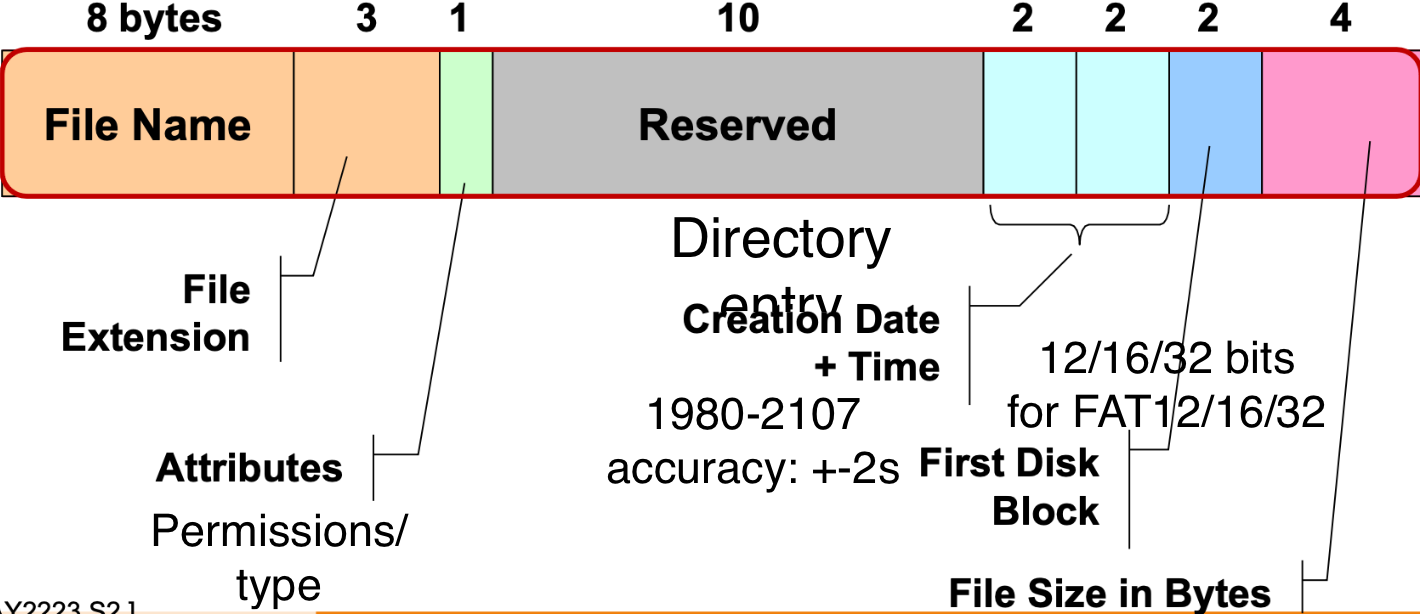
\includegraphics[scale=0.24]{directory-entry}
\end{itemize}

\subsection{Extended-2 FS (Ext2)}
\begin{itemize}
	\item Split into blocks (corresponding to 1 or more disk sectors) and grouped into Block Groups
	\begin{itemize}
		\item Data blks for same file should be in the same blk grp to reduce data fragmentation (spatial locality)
	\end{itemize}
	\item \keyword{I-Node}{Special structure describing each file/directory}
	\begin{itemize}
		\item Contains file metadata (access right, creation time etc) and data block add
	\end{itemize}
	\item \keyword{Superblock}{Describes whole FS including total num I-Node, I-Nodes per grp, total disk blocks + num in grps}
	\item \keyword{Group descriptors}{Describes block grp: num free blocks, num free I-Nodes, bitmap locations}
	\begin{itemize}
		\item Superblock and descriptors duplicated in each block group for redundancy
	\end{itemize}
	\item \keyword{Block\slash I-Node Bitmap}{Keep track usage status free(0)/occupied(1)}
	\item \keyword{I-Node Table}{Array of I-nodes in particular block group accessible by unique index}
\end{itemize}
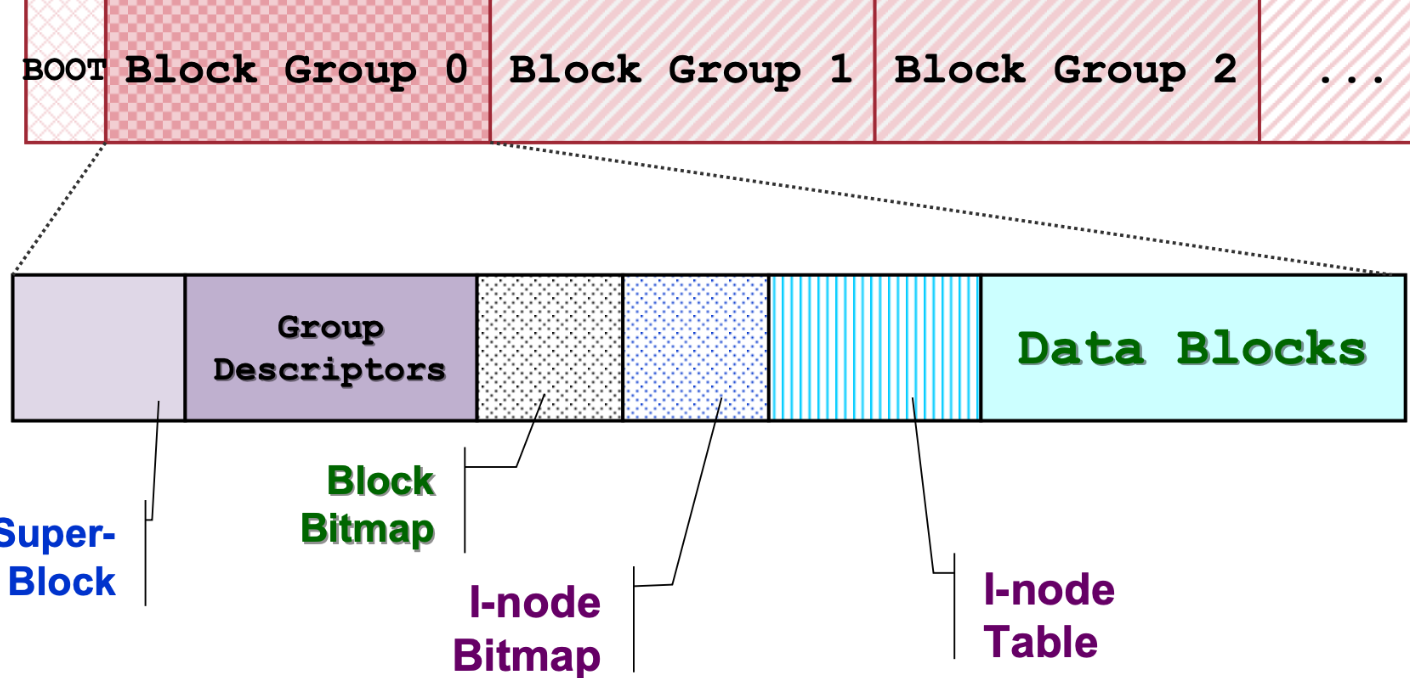
\includegraphics[scale=0.24]{ext2-fs-layout}
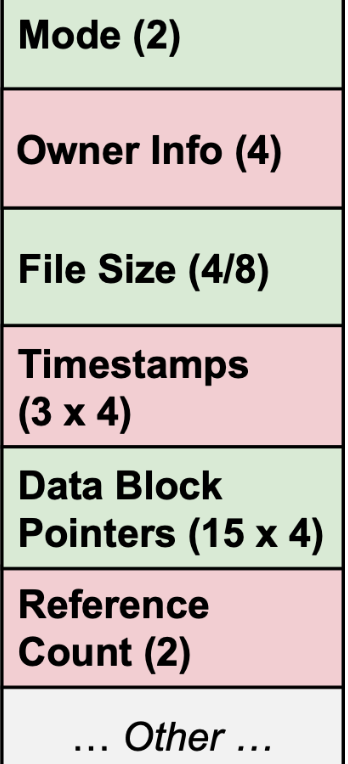
\includegraphics[scale=0.21]{i-node-table}

\subsubsection{I-Node Data Block Pointers (15)}
\begin{description}
	\item[Direct Block]{1st 12 pointers to actual data}
	\item[Single Indirect block]{13th pointer to a disk block full of direct pointers}
	\item[Double Indirect Block]{14th pointer to disk block full of single indirect blocks}
	\item[Triple Indirect Block]{15th pointer to block containing double indirect blocks}
\end{description}

\subsubsection{Directory Structure}
\begin{itemize}
	\item Data block of directory store linked list of directory entry
	\item \keyword{Directory entry}{Variable sized to store file/subdirectory info}
	\begin{itemize}
		\item I-Node number for file
		\item Size of this directory entry (to find next directory entry)
		\item Length of file/subdirectory name
		\item Type of file/subdirectory
		\item File/subdirectory name (up to 255 chars)
	\end{itemize}
\end{itemize}

\subsubsection{Open}
\begin{enumerate}
	\item Process P opens file /.../.../F which is located
	\begin{itemize}
		\item Split by "dir\slash" - If dir, locate directory entry in CurDir
		\item Retrieve I-Node number, read actual I-Node and continue from NewDir
		\item Else directly retrieve I-Node number and read actual I-Node
	\end{itemize}
	\item File info loaded into entry \textit{F} in sys-wide table and \textit{V} in I-Node table
	\item Create entry in P table to point to \textit{E} (file descriptor) and pointer from E to \textit{V} 
	\item Return file descriptor to caller
\end{enumerate}

\subsubsection{Deletion}
\begin{enumerate}
	\item Remove its directory entry from parent directory
	\begin{itemize}
		\item Point prev entry to next entry/end
		\item Blank record may be needed
	\end{itemize}
	\item Mark specific I-Node in bitmap as free
	\item Mark corresponding block in bitmap as free
\end{enumerate}

\subsubsection{Hard link}
\begin{itemize}
	\item New directory entry using same I-Node number as file
	\item Filename can be different
\end{itemize}
\begin{description}
	\item[Multiple references of I-Node]{Hard to determine when to delete I-Node}
	\begin{itemize}
		\item Maintain I-Node reference count
		\item Decrement for every deletion
	\end{itemize}
\end{description}
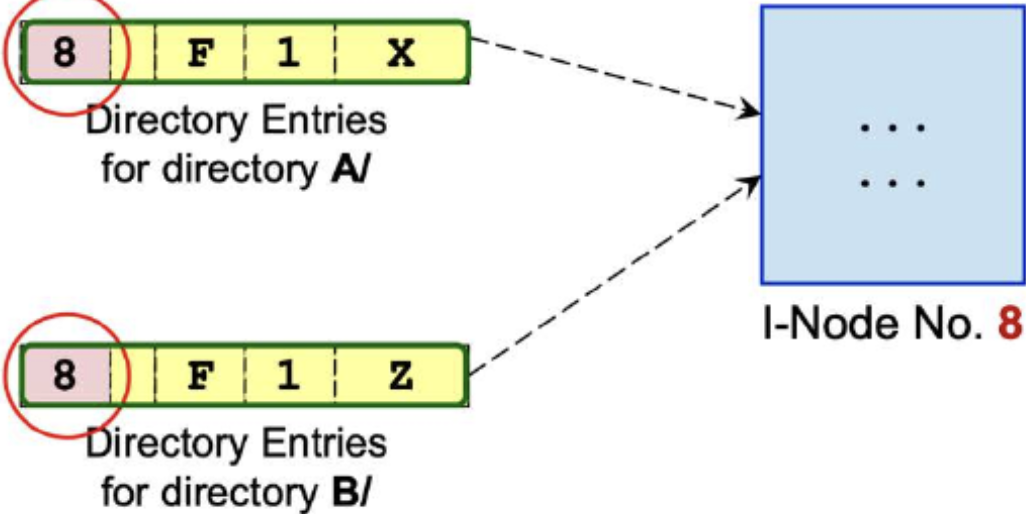
\includegraphics[scale=0.2]{hard-link}
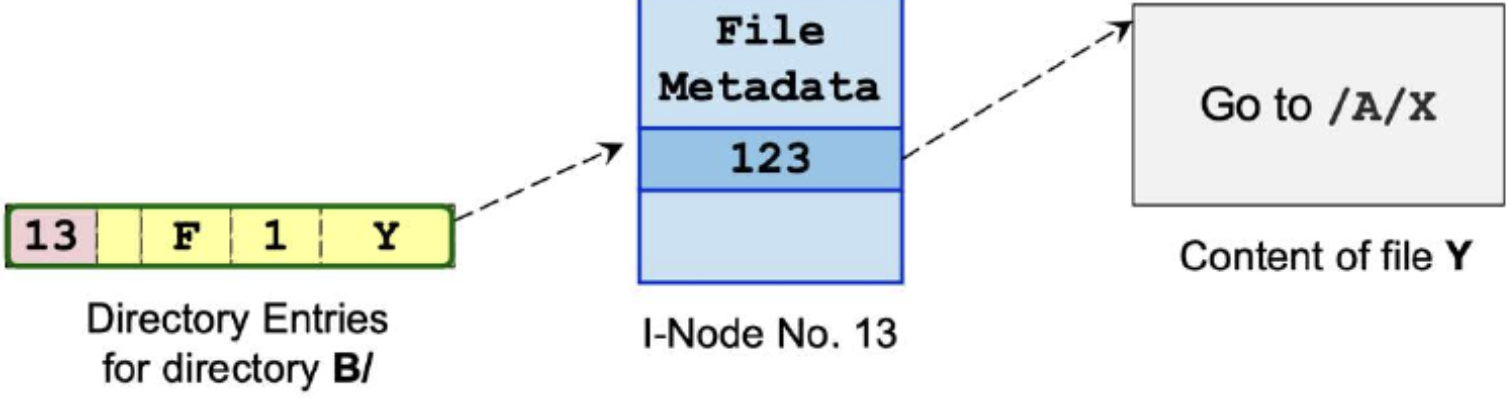
\includegraphics[scale=0.2]{sym-link}

\subsubsection{Sym Link}
\begin{itemize}
	\item File created with I-Node pointing to memory location of symlink
	\item Content of symlink == pathname of file
\end{itemize}
\begin{description}
	\item[Only pathname stored]{Link easily invalidated (during file name changes/deletion)}
\end{description}
\section{Finals}
\begin{itemize}
	\item Mapped file to SWAP will be dropped reread from file on disk
	\item Process opens 3 FD (STDIN, STDOUT, STDERR) auto upon initialization
\end{itemize}
\end{multicols*}
\end{small}
\end{document}
